% Options for packages loaded elsewhere
\PassOptionsToPackage{unicode}{hyperref}
\PassOptionsToPackage{hyphens}{url}
\PassOptionsToPackage{dvipsnames,svgnames,x11names}{xcolor}
%
\documentclass[
  letterpaper,
  DIV=11,
  numbers=noendperiod]{scrreprt}

\usepackage{amsmath,amssymb}
\usepackage{iftex}
\ifPDFTeX
  \usepackage[T1]{fontenc}
  \usepackage[utf8]{inputenc}
  \usepackage{textcomp} % provide euro and other symbols
\else % if luatex or xetex
  \usepackage{unicode-math}
  \defaultfontfeatures{Scale=MatchLowercase}
  \defaultfontfeatures[\rmfamily]{Ligatures=TeX,Scale=1}
\fi
\usepackage{lmodern}
\ifPDFTeX\else  
    % xetex/luatex font selection
\fi
% Use upquote if available, for straight quotes in verbatim environments
\IfFileExists{upquote.sty}{\usepackage{upquote}}{}
\IfFileExists{microtype.sty}{% use microtype if available
  \usepackage[]{microtype}
  \UseMicrotypeSet[protrusion]{basicmath} % disable protrusion for tt fonts
}{}
\makeatletter
\@ifundefined{KOMAClassName}{% if non-KOMA class
  \IfFileExists{parskip.sty}{%
    \usepackage{parskip}
  }{% else
    \setlength{\parindent}{0pt}
    \setlength{\parskip}{6pt plus 2pt minus 1pt}}
}{% if KOMA class
  \KOMAoptions{parskip=half}}
\makeatother
\usepackage{xcolor}
\setlength{\emergencystretch}{3em} % prevent overfull lines
\setcounter{secnumdepth}{5}
% Make \paragraph and \subparagraph free-standing
\makeatletter
\ifx\paragraph\undefined\else
  \let\oldparagraph\paragraph
  \renewcommand{\paragraph}{
    \@ifstar
      \xxxParagraphStar
      \xxxParagraphNoStar
  }
  \newcommand{\xxxParagraphStar}[1]{\oldparagraph*{#1}\mbox{}}
  \newcommand{\xxxParagraphNoStar}[1]{\oldparagraph{#1}\mbox{}}
\fi
\ifx\subparagraph\undefined\else
  \let\oldsubparagraph\subparagraph
  \renewcommand{\subparagraph}{
    \@ifstar
      \xxxSubParagraphStar
      \xxxSubParagraphNoStar
  }
  \newcommand{\xxxSubParagraphStar}[1]{\oldsubparagraph*{#1}\mbox{}}
  \newcommand{\xxxSubParagraphNoStar}[1]{\oldsubparagraph{#1}\mbox{}}
\fi
\makeatother

\usepackage{color}
\usepackage{fancyvrb}
\newcommand{\VerbBar}{|}
\newcommand{\VERB}{\Verb[commandchars=\\\{\}]}
\DefineVerbatimEnvironment{Highlighting}{Verbatim}{commandchars=\\\{\}}
% Add ',fontsize=\small' for more characters per line
\usepackage{framed}
\definecolor{shadecolor}{RGB}{241,243,245}
\newenvironment{Shaded}{\begin{snugshade}}{\end{snugshade}}
\newcommand{\AlertTok}[1]{\textcolor[rgb]{0.68,0.00,0.00}{#1}}
\newcommand{\AnnotationTok}[1]{\textcolor[rgb]{0.37,0.37,0.37}{#1}}
\newcommand{\AttributeTok}[1]{\textcolor[rgb]{0.40,0.45,0.13}{#1}}
\newcommand{\BaseNTok}[1]{\textcolor[rgb]{0.68,0.00,0.00}{#1}}
\newcommand{\BuiltInTok}[1]{\textcolor[rgb]{0.00,0.23,0.31}{#1}}
\newcommand{\CharTok}[1]{\textcolor[rgb]{0.13,0.47,0.30}{#1}}
\newcommand{\CommentTok}[1]{\textcolor[rgb]{0.37,0.37,0.37}{#1}}
\newcommand{\CommentVarTok}[1]{\textcolor[rgb]{0.37,0.37,0.37}{\textit{#1}}}
\newcommand{\ConstantTok}[1]{\textcolor[rgb]{0.56,0.35,0.01}{#1}}
\newcommand{\ControlFlowTok}[1]{\textcolor[rgb]{0.00,0.23,0.31}{\textbf{#1}}}
\newcommand{\DataTypeTok}[1]{\textcolor[rgb]{0.68,0.00,0.00}{#1}}
\newcommand{\DecValTok}[1]{\textcolor[rgb]{0.68,0.00,0.00}{#1}}
\newcommand{\DocumentationTok}[1]{\textcolor[rgb]{0.37,0.37,0.37}{\textit{#1}}}
\newcommand{\ErrorTok}[1]{\textcolor[rgb]{0.68,0.00,0.00}{#1}}
\newcommand{\ExtensionTok}[1]{\textcolor[rgb]{0.00,0.23,0.31}{#1}}
\newcommand{\FloatTok}[1]{\textcolor[rgb]{0.68,0.00,0.00}{#1}}
\newcommand{\FunctionTok}[1]{\textcolor[rgb]{0.28,0.35,0.67}{#1}}
\newcommand{\ImportTok}[1]{\textcolor[rgb]{0.00,0.46,0.62}{#1}}
\newcommand{\InformationTok}[1]{\textcolor[rgb]{0.37,0.37,0.37}{#1}}
\newcommand{\KeywordTok}[1]{\textcolor[rgb]{0.00,0.23,0.31}{\textbf{#1}}}
\newcommand{\NormalTok}[1]{\textcolor[rgb]{0.00,0.23,0.31}{#1}}
\newcommand{\OperatorTok}[1]{\textcolor[rgb]{0.37,0.37,0.37}{#1}}
\newcommand{\OtherTok}[1]{\textcolor[rgb]{0.00,0.23,0.31}{#1}}
\newcommand{\PreprocessorTok}[1]{\textcolor[rgb]{0.68,0.00,0.00}{#1}}
\newcommand{\RegionMarkerTok}[1]{\textcolor[rgb]{0.00,0.23,0.31}{#1}}
\newcommand{\SpecialCharTok}[1]{\textcolor[rgb]{0.37,0.37,0.37}{#1}}
\newcommand{\SpecialStringTok}[1]{\textcolor[rgb]{0.13,0.47,0.30}{#1}}
\newcommand{\StringTok}[1]{\textcolor[rgb]{0.13,0.47,0.30}{#1}}
\newcommand{\VariableTok}[1]{\textcolor[rgb]{0.07,0.07,0.07}{#1}}
\newcommand{\VerbatimStringTok}[1]{\textcolor[rgb]{0.13,0.47,0.30}{#1}}
\newcommand{\WarningTok}[1]{\textcolor[rgb]{0.37,0.37,0.37}{\textit{#1}}}

\providecommand{\tightlist}{%
  \setlength{\itemsep}{0pt}\setlength{\parskip}{0pt}}\usepackage{longtable,booktabs,array}
\usepackage{calc} % for calculating minipage widths
% Correct order of tables after \paragraph or \subparagraph
\usepackage{etoolbox}
\makeatletter
\patchcmd\longtable{\par}{\if@noskipsec\mbox{}\fi\par}{}{}
\makeatother
% Allow footnotes in longtable head/foot
\IfFileExists{footnotehyper.sty}{\usepackage{footnotehyper}}{\usepackage{footnote}}
\makesavenoteenv{longtable}
\usepackage{graphicx}
\makeatletter
\def\maxwidth{\ifdim\Gin@nat@width>\linewidth\linewidth\else\Gin@nat@width\fi}
\def\maxheight{\ifdim\Gin@nat@height>\textheight\textheight\else\Gin@nat@height\fi}
\makeatother
% Scale images if necessary, so that they will not overflow the page
% margins by default, and it is still possible to overwrite the defaults
% using explicit options in \includegraphics[width, height, ...]{}
\setkeys{Gin}{width=\maxwidth,height=\maxheight,keepaspectratio}
% Set default figure placement to htbp
\makeatletter
\def\fps@figure{htbp}
\makeatother
% definitions for citeproc citations
\NewDocumentCommand\citeproctext{}{}
\NewDocumentCommand\citeproc{mm}{%
  \begingroup\def\citeproctext{#2}\cite{#1}\endgroup}
\makeatletter
 % allow citations to break across lines
 \let\@cite@ofmt\@firstofone
 % avoid brackets around text for \cite:
 \def\@biblabel#1{}
 \def\@cite#1#2{{#1\if@tempswa , #2\fi}}
\makeatother
\newlength{\cslhangindent}
\setlength{\cslhangindent}{1.5em}
\newlength{\csllabelwidth}
\setlength{\csllabelwidth}{3em}
\newenvironment{CSLReferences}[2] % #1 hanging-indent, #2 entry-spacing
 {\begin{list}{}{%
  \setlength{\itemindent}{0pt}
  \setlength{\leftmargin}{0pt}
  \setlength{\parsep}{0pt}
  % turn on hanging indent if param 1 is 1
  \ifodd #1
   \setlength{\leftmargin}{\cslhangindent}
   \setlength{\itemindent}{-1\cslhangindent}
  \fi
  % set entry spacing
  \setlength{\itemsep}{#2\baselineskip}}}
 {\end{list}}
\usepackage{calc}
\newcommand{\CSLBlock}[1]{\hfill\break\parbox[t]{\linewidth}{\strut\ignorespaces#1\strut}}
\newcommand{\CSLLeftMargin}[1]{\parbox[t]{\csllabelwidth}{\strut#1\strut}}
\newcommand{\CSLRightInline}[1]{\parbox[t]{\linewidth - \csllabelwidth}{\strut#1\strut}}
\newcommand{\CSLIndent}[1]{\hspace{\cslhangindent}#1}

\KOMAoption{captions}{tableheading}
\makeatletter
\@ifpackageloaded{tcolorbox}{}{\usepackage[skins,breakable]{tcolorbox}}
\@ifpackageloaded{fontawesome5}{}{\usepackage{fontawesome5}}
\definecolor{quarto-callout-color}{HTML}{909090}
\definecolor{quarto-callout-note-color}{HTML}{0758E5}
\definecolor{quarto-callout-important-color}{HTML}{CC1914}
\definecolor{quarto-callout-warning-color}{HTML}{EB9113}
\definecolor{quarto-callout-tip-color}{HTML}{00A047}
\definecolor{quarto-callout-caution-color}{HTML}{FC5300}
\definecolor{quarto-callout-color-frame}{HTML}{acacac}
\definecolor{quarto-callout-note-color-frame}{HTML}{4582ec}
\definecolor{quarto-callout-important-color-frame}{HTML}{d9534f}
\definecolor{quarto-callout-warning-color-frame}{HTML}{f0ad4e}
\definecolor{quarto-callout-tip-color-frame}{HTML}{02b875}
\definecolor{quarto-callout-caution-color-frame}{HTML}{fd7e14}
\makeatother
\makeatletter
\@ifpackageloaded{bookmark}{}{\usepackage{bookmark}}
\makeatother
\makeatletter
\@ifpackageloaded{caption}{}{\usepackage{caption}}
\AtBeginDocument{%
\ifdefined\contentsname
  \renewcommand*\contentsname{Table of contents}
\else
  \newcommand\contentsname{Table of contents}
\fi
\ifdefined\listfigurename
  \renewcommand*\listfigurename{List of Figures}
\else
  \newcommand\listfigurename{List of Figures}
\fi
\ifdefined\listtablename
  \renewcommand*\listtablename{List of Tables}
\else
  \newcommand\listtablename{List of Tables}
\fi
\ifdefined\figurename
  \renewcommand*\figurename{Figure}
\else
  \newcommand\figurename{Figure}
\fi
\ifdefined\tablename
  \renewcommand*\tablename{Table}
\else
  \newcommand\tablename{Table}
\fi
}
\@ifpackageloaded{float}{}{\usepackage{float}}
\floatstyle{ruled}
\@ifundefined{c@chapter}{\newfloat{codelisting}{h}{lop}}{\newfloat{codelisting}{h}{lop}[chapter]}
\floatname{codelisting}{Listing}
\newcommand*\listoflistings{\listof{codelisting}{List of Listings}}
\makeatother
\makeatletter
\makeatother
\makeatletter
\@ifpackageloaded{caption}{}{\usepackage{caption}}
\@ifpackageloaded{subcaption}{}{\usepackage{subcaption}}
\makeatother

\ifLuaTeX
  \usepackage{selnolig}  % disable illegal ligatures
\fi
\usepackage{bookmark}

\IfFileExists{xurl.sty}{\usepackage{xurl}}{} % add URL line breaks if available
\urlstyle{same} % disable monospaced font for URLs
\hypersetup{
  pdftitle={Geographic Data Science for Applied Economists},
  pdfauthor={Dr.~Carmen Cabrera-Arnau},
  colorlinks=true,
  linkcolor={blue},
  filecolor={Maroon},
  citecolor={Blue},
  urlcolor={Blue},
  pdfcreator={LaTeX via pandoc}}


\title{Geographic Data Science for Applied Economists}
\author{Dr.~Carmen Cabrera-Arnau}
\date{2024-09-26}

\begin{document}
\maketitle

\renewcommand*\contentsname{Table of contents}
{
\hypersetup{linkcolor=}
\setcounter{tocdepth}{2}
\tableofcontents
}

\bookmarksetup{startatroot}

\chapter*{Welcome}\label{welcome}
\addcontentsline{toc}{chapter}{Welcome}

\markboth{Welcome}{Welcome}

This is the website for the ``Geographic Data Science'' module
\textbf{ENVS363/563} at the University of Liverpool. This is course
designed and delivered by Dr.~Elisabetta Pietrostefani and Dr.~Carmen
Cabrera-Arnau from the Geographic Data Science Lab at the University of
Liverpool, United Kingdom. Much of the course material is inspired by
Dani Arribas-Bel's
\href{https://darribas.org/gds_course/content/home.html}{course on
Geographic Data Science}.

This module will introduce students to the field of \textbf{Geographic
Data Science (GDS)}, a discipline established at the intersection
between Geographic Information Science (GIS) and Data Science. The
course covers how the modern GIS toolkit can be integrated with Data
Science tools to solve practical real-world problems.

Core to the set of employable skills to be taught in this course is an
introduction to programming tools. Students will be able to whether to
develop their skills in either R or Python in Lab sessions.

The website is \textbf{free to use} and is licensed under the
\href{https://creativecommons.org/licenses/by-nc-nd/4.0/}{Attribution-NonCommercial-NoDerivatives
4.0 International}. A compilation of this web course is hosted as a
GitHub repository that you can access:

\begin{itemize}
\tightlist
\item
  As an \href{https://pietrostefani.github.io/gds/}{html website}.
\item
  As a \href{https://github.com/pietrostefani/gds}{GitHub repository}.
\end{itemize}

\section*{Contact}\label{contact}
\addcontentsline{toc}{section}{Contact}

\markright{Contact}

\begin{quote}
Elisabetta Pietrostefani - Module Leader - e.pietrostefani {[}at{]}
liverpool.ac.uk Lecturer in Geographic Data Science, Roxby Building,
University of Liverpool - 74 Bedford St S, Liverpool, L69 7ZT, United
Kingdom.
\end{quote}

\begin{quote}
Carmen Cabrera-Arnau - c.cabrera-arnau {[}at{]} liverpool.ac.uk Lecturer
in Geographic Data Science, Roxby Building, University of Liverpool - 74
Bedford St S, Liverpool, L69 7ZT, United Kingdom.
\end{quote}

\part{Overview}

\section*{Aims}\label{aims}
\addcontentsline{toc}{section}{Aims}

\markright{Aims}

The module has three main aims.

\begin{itemize}
\item
  Provide students with core competences in Geographic Data Science
  (GDS). This includes advancing their statistical and numerical
  literacy and introducing basic principles of programming and
  state-of-the-art computational tools for GDS;
\item
  Present a comprehensive overview of the main methodologies available
  to the Geographic Data Scientist, as well as their intuition as to how
  and when they can be applied;
\item
  Focus on real world applications of these techniques in a geographical
  and applied context.
\end{itemize}

\section*{Learning Outcomes}\label{learning-outcomes}
\addcontentsline{toc}{section}{Learning Outcomes}

\markright{Learning Outcomes}

By the end of the module, students should be able to:

\textbf{For all}

\begin{enumerate}
\def\labelenumi{(\arabic{enumi})}
\item
  Demonstrate advanced GIS/GDS concepts and be able to use the tools
  programmatically to import, manipulate and analyse data in different
  formats.
\item
  Understand the motivation and inner workings of the main
  methodological approaches of GDS, both analytical and visual.
\item
  Evaluate the suitability of a specific technique, what it can offer
  and how it can help answer questions of interest.
\item
  Apply a number of spatial analysis techniques and how to interpret the
  results, in the process of turning data into information.
\item
  When faced with a new data-set, work independently using GIS/GDS tools
  programmatically.
\end{enumerate}

\textbf{Only for MSc students}

\begin{enumerate}
\def\labelenumi{\arabic{enumi}.}
\setcounter{enumi}{5}
\tightlist
\item
  Demonstrate a sound understanding of how real-world (geo)data are
  produced, their potential insights and biases, as well as
  opportunities and limitations.
\end{enumerate}

\section*{Feedback}\label{feedback}
\addcontentsline{toc}{section}{Feedback}

\markright{Feedback}

\emph{Formal assessment of one map and one computational essays}.
Written assignment-specific feedback will be provided within three
working weeks of the submission deadline. Comments will offer an
understanding of the mark awarded and identify areas which can be
considered for improvement in future assignments.

\emph{Verbal face-to-face feedback}. Immediate face-to-face feedback
will be provided during computer, discussion and clinic sessions in
interaction with staff. This will take place in all live sessions during
the semester.

\emph{Online forum}. Asynchronous written feedback will be provided via
an online forum. Students are encouraged to contribute by asking and
answering questions relating to the module content. Staff will monitor
the forum Monday to Friday 9am-5pm, but it will be open to students to
make contributions at all times. Response time will vary depending on
the complexity of the question and staff availability.

\chapter*{Environment}\label{environment}
\addcontentsline{toc}{chapter}{Environment}

\markboth{Environment}{Environment}

This course can be followed by anyone with access to a bit of technical
infrastructure. This section details the set of local and online
requirements you will need to be able to follow along, as well as
instructions or pointers to get set up on your own. This is a
centralised section that lists \emph{everything} you will require.

\section*{Coding Languages}\label{coding-languages}
\addcontentsline{toc}{section}{Coding Languages}

\markright{Coding Languages}

In this course, you have the option to follow along using either
\texttt{R} or \texttt{Python}, depending on your past experience with
these programming languages and preference. Please choose \textbf{one}
language to focus on and stick to it throughout.

\begin{itemize}
\item
  If you want to follow the course in \texttt{R}, you can find
  instructions to set up your environment
  \href{https://pietrostefani.github.io/gds/environR.html}{here}.
\item
  If you want to follow the course in \texttt{Python}, you can find
  instructions to set up your environment
  \href{https://pietrostefani.github.io/gds/environPy.html}{here}.
\end{itemize}

This course has two assignments and you will be required to submit both
assignments in the same programming languages. The next two sections
will guide you through the process of setting up your development
environment in \texttt{R} or \texttt{Python}, so you can get started
with the course smoothly.

\section*{Reproducing code in this
book}\label{reproducing-code-in-this-book}
\addcontentsline{toc}{section}{Reproducing code in this book}

\markright{Reproducing code in this book}

If you want to reproduce the code in the book, you need the most recent
version of Quarto, R and relevant packages. These can be installed
following the instructions provided in our
\href{https://gdsl-ul.github.io/r_install/}{R installation guide}.
Quarto (1.2.280) can be downloaded from
\href{https://quarto.org/docs/get-started/}{the Quarto website}, it may
already be installed when you download R and R Studio.

\chapter*{Python}\label{python}
\addcontentsline{toc}{chapter}{Python}

\markboth{Python}{Python}

To run the analysis and reproduce the code in Python, you will need to
set up the Python environment to:

\begin{itemize}
\tightlist
\item
  Execute the \href{https://docs.jupyter.org/en/latest/}{Jupyter
  Notebooks} of the Lab sessions of the course.
\item
  Prepare your own Jupyter Notebooks for the assignments.
\end{itemize}

\begin{tcolorbox}[enhanced jigsaw, breakable, toptitle=1mm, titlerule=0mm, opacityback=0, colback=white, coltitle=black, leftrule=.75mm, bottomtitle=1mm, colframe=quarto-callout-important-color-frame, colbacktitle=quarto-callout-important-color!10!white, toprule=.15mm, bottomrule=.15mm, arc=.35mm, rightrule=.15mm, opacitybacktitle=0.6, title=\textcolor{quarto-callout-important-color}{\faExclamation}\hspace{0.5em}{Important}, left=2mm]

\textbf{Do not} try to run Python code in RStudio. Only run in Jupyter
Notebooks (.ipynb) with the Python environment provided.

\end{tcolorbox}

We will use \texttt{Miniconda} to handle our working environment.

\section*{Set up Miniconda (and Python) on Ms
Windows}\label{set-up-miniconda-and-python-on-ms-windows}
\addcontentsline{toc}{section}{Set up Miniconda (and Python) on Ms
Windows}

\markright{Set up Miniconda (and Python) on Ms Windows}

\subsection*{Installation}\label{installation}
\addcontentsline{toc}{subsection}{Installation}

\begin{enumerate}
\def\labelenumi{\arabic{enumi}.}
\item
  Install Miniconda:

  \begin{itemize}
  \item
    \textbf{Option 1}: On a UoL Machine: Anaconda is installed on many
    university machines. Please check whether it is installed. If not,
    download and install Anaconda through from
    \texttt{Install\ University\ Applications}, type and choose
    \texttt{Anaconda}.
  \item
    \textbf{Option 2}: \emph{Recommended} - Install Miniconda on your
    personal Laptop: Follow the instructions
    \href{https://docs.conda.io/projects/miniconda/en/latest/miniconda-install.html}{here}.
  \end{itemize}
\item
  During the installation, leave the default settings. In particular,
  when asked whom to ``Install Miniconda for'', choose ``Just for me''.
\end{enumerate}

\begin{tcolorbox}[enhanced jigsaw, breakable, toptitle=1mm, titlerule=0mm, opacityback=0, colback=white, coltitle=black, leftrule=.75mm, bottomtitle=1mm, colframe=quarto-callout-caution-color-frame, colbacktitle=quarto-callout-caution-color!10!white, toprule=.15mm, bottomrule=.15mm, arc=.35mm, rightrule=.15mm, opacitybacktitle=0.6, title=\textcolor{quarto-callout-caution-color}{\faFire}\hspace{0.5em}{University Machines}, left=2mm]

If you do choose to work on University Machines

\begin{enumerate}
\def\labelenumi{\arabic{enumi}.}
\tightlist
\item
  Chose a machine where Anaconda has been pre-installed.
\item
  Always use the same machine. For example if on the first day you are
  using CT60 Station 17 - Orange Zone, continue using this machine for
  the rest of the course. If you change machine you will need to
  re-install the environment every time.
\end{enumerate}

\end{tcolorbox}

\subsection*{Set up the Directories}\label{set-up-the-directories}
\addcontentsline{toc}{subsection}{Set up the Directories}

\begin{enumerate}
\def\labelenumi{\arabic{enumi}.}
\tightlist
\item
  Create a folder where you want to keep your work conducted throughout
  this course. For example, call it \texttt{envs363\_563}. You can save
  it wherever you want. If you are working on a university machine, it
  could be worth creating it in \texttt{M:/}, which is your ``virtual''
  hard-disk.
\end{enumerate}

\begin{enumerate}
\def\labelenumi{\arabic{enumi}.}
\setcounter{enumi}{1}
\tightlist
\item
  Download the
  \href{https://github.com/pietrostefani/gds/tree/main/data}{data} to
  run and render the jupyter notebooks. To learn how to download folders
  from github see
  \href{https://pietrostefani.github.io/gds/download.html}{here}.
\item
  Unzip the folders and move the nested folders into the folder
  \texttt{envs363\_563}.
\item
  Create another folder called \texttt{labs}
\end{enumerate}

The folder structure should look like:

\begin{verbatim}
envs363_563/
├── data/
└── labs/
\end{verbatim}

\subsection*{Set up the Python
Environment}\label{set-up-the-python-environment}
\addcontentsline{toc}{subsection}{Set up the Python Environment}

\begin{enumerate}
\def\labelenumi{\arabic{enumi}.}
\tightlist
\item
  Download the \texttt{envs363\_563.yml} from GitHub by cliciking
  \texttt{Download\ raw\ file}, top right
  \href{https://github.com/pietrostefani/gds/blob/main/envs363-563.yml}{at
  this page}
\item
  Save it in the folder \texttt{envs363\_563} created before.
\item
  Type in the search bar and find the
  \texttt{Anaconda\ Powershell\ Prompt} if working on University Machine
  or \texttt{Anaconda\ Prompt\ (miniconda\ 3)} if on your personal.
  Launch it. The terminal should appear.
\end{enumerate}

\begin{enumerate}
\def\labelenumi{\arabic{enumi}.}
\setcounter{enumi}{2}
\tightlist
\item
  In the \textbf{Anaconda Terminal} write:
  \texttt{conda\ env\ create\ -n\ envs363\_563\ -\/-file\ M:\textbackslash{}envs363\textbackslash{}envs363\_563.yml}
  and press \texttt{Enter}; if the file is located elsewhere you'll need
  to use the corresponding file path.
\item
  If you are prompted any questions, press \texttt{y}. This process will
  install all the packages necessary to carry out the lab sessions.
\item
  In the \textbf{Anaconda Terminal} write
  \texttt{conda\ activate\ envs363\_563} and press \texttt{Enter}. This
  activates your working environment.
\end{enumerate}

\begin{enumerate}
\def\labelenumi{\arabic{enumi}.}
\setcounter{enumi}{5}
\tightlist
\item
  \emph{Necessary} on University machines, otherwise \emph{Optional}:
  Configuration of Jupyter Notebooks

  \begin{itemize}
  \tightlist
  \item
    In the \textbf{Anaconda Terminal}, write
    \texttt{jupyter\ server\ -\/-generate-config} and press enter. This,
    at least in Windows, should create a file to:
    \texttt{C:\textbackslash{}Users\textbackslash{}username\textbackslash{}.jupyter\textbackslash{}jupyter\_server\_config.py}.
  \item
    Open the file with a text editor
    (e.g.~\href{https://notepad-plus-plus.org}{Notepad++}), do a
    \texttt{ctrl-f} search for: \texttt{c.ServerApp.root\_dir},
    uncomment it by removing the \# and change it to
    \texttt{c.ServerApp.notebook\_dir\ =\ \textquotesingle{}M:\textbackslash{}\textbackslash{}your\textbackslash{}\textbackslash{}new\textbackslash{}\textbackslash{}path},
    for example the directory where you created the
    \texttt{envs363\_563} folder. In the University Machines, it is
    advised to work on the directory \texttt{M:\textbackslash{}}.
  \item
    Save the file and close it.
  \end{itemize}
\end{enumerate}

\subsection*{Start a Lab Session}\label{start-a-lab-session}
\addcontentsline{toc}{subsection}{Start a Lab Session}

\begin{enumerate}
\def\labelenumi{\arabic{enumi}.}
\tightlist
\item
  Download the Jupyter Notebook of the session in your folder. Choose
  one jupyter notebook and click \texttt{Dowload\ raw\ file} as shown
  below.
\end{enumerate}

\begin{enumerate}
\def\labelenumi{\arabic{enumi}.}
\setcounter{enumi}{1}
\tightlist
\item
  Save the file in the \texttt{labs} folder within your
  \texttt{envs363\_563} folder on your machine.
\item
  Type in the search bar, find and open the
  \texttt{Anaconda\ Prompt\ (miniconda\ 3)}.
\item
  In the \textbf{Anaconda Terminal} write and run
  \texttt{conda\ activate\ envs363\_563}.
\item
  In the \textbf{Anaconda Terminal} write and run
  \texttt{jupyter\ notebook}. This should open Jupyter Notebook in your
  default browser.
\end{enumerate}

\begin{enumerate}
\def\labelenumi{\arabic{enumi}.}
\setcounter{enumi}{5}
\tightlist
\item
  Navigate to your course folder in and double click on the notebook
  downloaded in step 1.
\item
  You can now work on your copy of the notebook.
\end{enumerate}

Follow these instructions and test your installation \textbf{prior to
the first Lab Session}. If you experience any issues, write a message on
the Ms Teams channel of the module. Setting up the Python environment is
necessary for:

\begin{itemize}
\tightlist
\item
  Executing the \href{https://docs.jupyter.org/en/latest/}{Jupyter
  Notebooks} of the Lab sessions of the course.
\item
  Preparing your own Jupyter Notebooks for the assignments (one each).
\end{itemize}

\section*{Set up Miniconda (and Python) on
MAC}\label{set-up-miniconda-and-python-on-mac}
\addcontentsline{toc}{section}{Set up Miniconda (and Python) on MAC}

\markright{Set up Miniconda (and Python) on MAC}

\subsection*{Installation}\label{installation-1}
\addcontentsline{toc}{subsection}{Installation}

To install Miniconda on your personal laptop, Follow the instructions
\href{https://docs.conda.io/projects/miniconda/en/latest/miniconda-install.html}{here}.
During the installation, leave the default settings. In particular, when
asked whom to ``Install Miniconda for'', choose ``Just for me''.

\subsection*{Set up the Directories}\label{set-up-the-directories-1}
\addcontentsline{toc}{subsection}{Set up the Directories}

\begin{enumerate}
\def\labelenumi{\arabic{enumi}.}
\tightlist
\item
  Create a folder where you want to keep your work conducted throughout
  this course. For example, call it \texttt{envs363\_563}. You can save
  it wherever you want. For example, Elisabetta has named her folder
  \texttt{envs363\_563} and it's in her Dropbox in
  \texttt{Users/PIETROST/Library/CloudStorage/Dropbox/envs363\_563}
\item
  Download the
  \href{https://github.com/pietrostefani/gds/tree/main/data}{data} to
  run and render the jupyter notebooks. To learn how to download folders
  from github see
  \href{https://pietrostefani.github.io/gds/download.html}{here}.
\item
  Unzip the folders and move the nested folders into the folder
  \texttt{envs363\_563}.
\item
  Create another folder called \texttt{labs}
\end{enumerate}

The folder structure should look like:

\begin{verbatim}
envs363_563/ ├── data/ └── labs/
\end{verbatim}

\subsection*{Set up the Python
Environment}\label{set-up-the-python-environment-1}
\addcontentsline{toc}{subsection}{Set up the Python Environment}

\begin{enumerate}
\def\labelenumi{\arabic{enumi}.}
\tightlist
\item
  Download the \texttt{envs363\_563.yml} from GitHub by clicking
  \texttt{Download\ raw\ file}, top right
  \href{https://github.com/pietrostefani/gds/blob/main/envs363-563.yml}{at
  this page}
\item
  Save it in the folder \texttt{envs363\_563} created before.
\item
  Type in the search bar and open the \textbf{Terminal}.
\item
  In the \textbf{Terminal} write
  \texttt{conda\ env\ create\ -n\ envs363\ -\/-file\ envs363\_563.yml}
  and press \texttt{Enter}. This will need to be modified according to
  where you placed the \texttt{envs363\_563} folder. For example,
  Elisabetta has named her folder \texttt{envs363\_563} and it's in her
  Dropbox in
  \texttt{Users/PIETROST/Library/CloudStorage/Dropbox/envs363\_563/envs363\_563.yml}.
  If you created the \texttt{envs363\_563} folder on your desktop, the
  path would be \texttt{Desktop/envs363\_563}.
\end{enumerate}

\begin{enumerate}
\def\labelenumi{\arabic{enumi}.}
\setcounter{enumi}{3}
\tightlist
\item
  If you are prompted any questions, press \texttt{y}. This process will
  install all the packages necessary to carry out the lab sessions.
\item
  You should then see this
\end{enumerate}

\subsection*{Start a Lab Session}\label{start-a-lab-session-1}
\addcontentsline{toc}{subsection}{Start a Lab Session}

\begin{enumerate}
\def\labelenumi{\arabic{enumi}.}
\tightlist
\item
  Download the Jupyter Notebook of the session in your folder. Choose
  one jupyter notebook and click \texttt{Dowload\ raw\ file} as shown
  below
\end{enumerate}

\begin{enumerate}
\def\labelenumi{\arabic{enumi}.}
\setcounter{enumi}{1}
\tightlist
\item
  Save the file in the \texttt{labs} folder within your \texttt{envs363}
  folder on your machine.
\item
  Type in the search bar, find and open the \textbf{Terminal}.
\item
  In the \textbf{Terminal} write and run
  \texttt{conda\ activate\ envs363}.
\item
  In the \textbf{Terminal} write and run \texttt{jupyter\ notebook}.
\end{enumerate}

\begin{enumerate}
\def\labelenumi{\arabic{enumi}.}
\setcounter{enumi}{5}
\tightlist
\item
  This should open Jupyter Notebook in your default browser. You should
  see something like this:
\end{enumerate}

\begin{enumerate}
\def\labelenumi{\arabic{enumi}.}
\setcounter{enumi}{6}
\tightlist
\item
  Navigate to your folder. You can now work on your copy of the
  notebook.
\end{enumerate}

\section*{Py Basics}\label{py-basics}
\addcontentsline{toc}{section}{Py Basics}

\markright{Py Basics}

Please refer to the tutorials from
\href{https://www.learnpython.org/en/Welcome}{learnpython.org} for an
introduction to coding in Python. We particularly recommend the
tutorials listed under the ``Learn the Basics'' section.

\section*{Resources}\label{resources}
\addcontentsline{toc}{section}{Resources}

\markright{Resources}

Some help along the way with:

\begin{enumerate}
\def\labelenumi{\arabic{enumi}.}
\item
  \href{https://geographicdata.science/book/intro.html}{Geographic Data
  Science with Python}.
\item
  \href{https://pythongis.org/index.html}{Python for Geographic Data
  Analysis}
\end{enumerate}

\chapter*{Download data from github}\label{download-data-from-github}
\addcontentsline{toc}{chapter}{Download data from github}

\markboth{Download data from github}{Download data from github}

\begin{enumerate}
\def\labelenumi{\arabic{enumi}.}
\tightlist
\item
  Go to \url{https://download-directory.github.io}
\end{enumerate}

\begin{enumerate}
\def\labelenumi{\arabic{enumi}.}
\setcounter{enumi}{1}
\tightlist
\item
  Go to the folder you need for your Lab. For example copy:
  \url{https://github.com/pietrostefani/gds/tree/main/data/London}
\end{enumerate}

\begin{enumerate}
\def\labelenumi{\arabic{enumi}.}
\setcounter{enumi}{2}
\item
  Paste it in the green box\ldots{} give it a few minutes
\item
  Check your downloads file and unzip
\end{enumerate}

\part{1 Introduction}

In this section we introduce what Geographic Data Science is. We top it
up with a few (optional) further readings for the interested and curious
mind.

Slides can be downloaded \href{./html/introduction_gds.pdf}{``here''}

\section*{From Geographic Information Systems to Geographic Data
Science}\label{from-geographic-information-systems-to-geographic-data-science}
\addcontentsline{toc}{section}{From Geographic Information Systems to
Geographic Data Science}

\markright{From Geographic Information Systems to Geographic Data
Science}

Geographic Information holds a pivotal position within our modern
societies, permeating various aspects of our daily lives. It underpins
essential sectors such as housing, transportation, insurance, banking,
telecommunications, logistics, energy, retail, agriculture, healthcare,
and urban planning. Its significance lies in the capacity to analyze and
derive invaluable insights from geo-spatial data, enabling us to make
informed decisions and address complex challenges. Proficiency in this
field equips individuals with the ability to work with real-world data
across multiple domains and tackle diverse problems. Furthermore, it
provides the opportunity to acquire essential data science skills and
utilize important tools for answering spatial questions. Given its
wide-ranging applications and the increasing reliance on location-based
information, there is a substantial demand for experts in the geographic
information industry, making it a highly sought-after skill set in
today's workforce.

\textbf{What information does GIS use?}

\begin{itemize}
\tightlist
\item
  Data that defines geographical features like roads, rivers
\item
  Soil types, land use, elevation
\item
  Demographics, socioeconomic attributes
\item
  Environmental, climate, air-quality
\item
  Annotations that label features and places
\end{itemize}

From the real-world to the GIS world

\includegraphics[width=0.8\textwidth,height=\textheight]{./img/layers.png}

\textbf{Geographic Data Science}

A GIS person typically produces cartographic and analytical products
using desktop software. A geospatial data scientist \textbf{creates
code} and \textbf{runs pipelines} that produce \textbf{analytical
products} and \textbf{cartographic representations}.

This entails working with real-world data from various domains and
tackling a wide range of complex problems. Through this process
geospatial data science includes both data science and GIS tools that
lead to the analysos of intricate spatial questions effectively. The
synergy between CyberGIS and Geographic Data Science is unmistakable,
with coding playing a pivotal role in enabling the seamless development
of interactive data analysis. By leveraging cutting-edge technologies
and innovative methodologies, this symbiotic relationship enhances the
accessibility, scalability, and interactivity of geospatial data
analysis. Consequently, it opens up new vistas for collaborative
research and decision-making processes.

This multifaceted approach equips them with the knowledge and expertise
to navigate the intricate world of spatial data analysis and contribute
meaningfully to diverse fields where location-based insights are
invaluable.

\includegraphics[width=0.8\textwidth,height=\textheight]{./img/gds.png}

\section*{What is Geographic Data
Science?}\label{what-is-geographic-data-science}
\addcontentsline{toc}{section}{What is Geographic Data Science?}

\markright{What is Geographic Data Science?}

Statistician George Box :

\emph{All models are wrong, but some are useful In a similar fashion.}

Geographer Keith Ord :

\emph{All maps are wrong, but some are useful.}

\section*{Open Source GIS}\label{open-source-gis}
\addcontentsline{toc}{section}{Open Source GIS}

\markright{Open Source GIS}

\textbf{Open source Geographic Information Systems (GIS)}, such as
\textbf{QGIS}, have made geographic analysis accessible worldwide. GIS
programs tend to emphasize graphical user interfaces (GUIs), with the
unintended consequence of discouraging reproducibility (although many
can be used from the command line Python + QGIS). \textbf{R} and
\textbf{Python} by contrast, emphasizes the command line interface
(CLI).

The \textbf{`geodata revolution'} drives demand for high performance
computer hardware and efficient, scalable software to handle and extract
signal from the noise, to understand and perhaps change the world.
Spatial databases enable storage and generation of manageable subsets
from the vast geographic data stores, making interfaces for gaining
knowledge from them vital tools for the future.

\textbf{R} and \textbf{Python} are both tools with advanced modeling and
visualization capabilities.

\section*{\texorpdfstring{\textbf{Open
Science}}{Open Science}}\label{open-science}
\addcontentsline{toc}{section}{\textbf{Open Science}}

\markright{\textbf{Open Science}}

Why do we care about the processes and tools we use when we do
computational work? Where do the current paradigm come from? Are we on
the verge of a new model? For all of this, we we have two reads to set
the tone. Make sure to get those in first thing before moving on to the
next bits.

\begin{itemize}
\item
  First half of Chapter 1 in ``Geographic Data Science with Python''
  \href{https://geographicdata.science/book/notebooks/01_geo_thinking.html}{Geographic
  Thinking for Data Scientists}.
\item
  The 2018 Atlantic piece
  \href{https://juliacomputing.com/docs/press_pdfs/april5.pdf}{``The
  scientific paper is obsolete''} on computational notebooks, by James
  Somers.
\end{itemize}

\section*{\texorpdfstring{\textbf{Modern Scientific
Tools}}{Modern Scientific Tools}}\label{modern-scientific-tools}
\addcontentsline{toc}{section}{\textbf{Modern Scientific Tools}}

\markright{\textbf{Modern Scientific Tools}}

Once we know a bit more about why we should care about the tools we use,
let's dig into those that will underpin much of this course. This part
is interesting in itself, but will also valuable to better understand
the practical aspects of the course. Again, we have two reads here to
set the tone and complement the practical introduction we saw in the
Hands-on and DIY parts of the previous block. We are closing the circle
here:

\begin{itemize}
\tightlist
\item
  Second half of Chapter 1 in ``Geographic Data Science with Python''
  \href{https://geographicdata.science/book/notebooks/01_geo_thinking.html}{Geographic
  Thinking for Data Scientists}.
\end{itemize}

\part{\textbf{Further readings}}

Watch:
\href{https://www.sciencefriday.com/segments/solving-lifes-everyday-problems-with-data/}{Solving
Life's Everyday Problems with Data}

\begin{enumerate}
\def\labelenumi{\arabic{enumi}.}
\item
  \textbf{``Doing Data Science''} by Cathy O'Neil, Rachel Schutt in
  \href{http://shop.oreilly.com/product/0636920028529.do}{html} or
  \href{http://cdn.oreillystatic.com/oreilly/booksamplers/9781449358655_sampler.pdf}{pdf}
  is a general overview of why we needed Data Science and where if came
  from.
\item
  A slightly more technical historical perspective on where Data Science
  came from and where it might go can be found in David Donoho's recent
  overview
  \href{https://www.tandfonline.com/doi/full/10.1080/10618600.2017.1384734}{\textbf{``50
  years of Data Science''}}.
\item
  A geographic take on Data Science, proposing more interaction between
  Geography and Data Science is Alex Singelton's and Dani Arribas-Bel's
  \href{https://onlinelibrary.wiley.com/doi/full/10.1111/gean.12194}{\textbf{Geographic
  Data Science}} article.
\end{enumerate}

\chapter*{OpenScience in Python}\label{sec-open-science-Python}
\addcontentsline{toc}{chapter}{OpenScience in Python}

\markboth{OpenScience in Python}{OpenScience in Python}

Now that you know what computational notebooks are and why we should
care about them, let's start using them! This section introduces you to
using Python for manipulating tabular data. Please read through it
carefully and pay attention to how ideas about manipulating data are
translated into code. For this part, you can read directly from the
course website, although it is recommended you follow the section
interactively by running the code on your own.

Once you have read through, jump on the
\href{https://pietrostefani.github.io/gds/openscienceDIY.html}{Do-It-Yourself}
section, which will provide you with a challenge that you should
complete on your own, and will allow you to put what you have already
learnt into practice.

\section*{Data wrangling}\label{data-wrangling}
\addcontentsline{toc}{section}{Data wrangling}

\markright{Data wrangling}

Real world datasets tend to be messy. There is no way around it:
datasets have ``holes'' (missing data), the amount of formats in which
data can be stored is endless, and the best structure to share data is
not always the optimum to analyze them, hence the need to wrangle
(manipulate, transform and structure) them. As has been correctly
pointed out in many outlets
(\href{https://www.nytimes.com/2014/08/18/technology/for-big-data-scientists-hurdle-to-insights-is-janitor-work.html?_r=0}{e.g.}),
much of the
\href{https://twitter.com/BigDataBorat/status/306596352991830016}{time}
spent in what is called (Geo-)Data Science is related not only to
sophisticated modeling and insight, but to more basic and less exotic
tasks such as obtaining data, processing, turning them into a shape that
makes analysis possible, and exploring it to get to know their basic
properties.

In this session, you will use a few real world datasets and learn how to
process them in Python so they can be transformed and manipulated, if
necessary, and analyzed. For this, we will introduce some of the
fundamental tools of data analysis and scientific computing. We use a
prepared dataset that saves us much of the more intricate processing
that goes beyond the introductory level the session is aimed at.

In this notebook, we discuss several patterns to clean and structure
data properly, including tidying, subsetting, and aggregating; and we
finish with some basic visualization. An additional extension presents
more advanced tricks to manipulate tabular data.

Before we get our hands data-dirty, let us import all the additional
libraries we will need to run the code:

\section*{Loading packages}\label{loading-packages}
\addcontentsline{toc}{section}{Loading packages}

\markright{Loading packages}

We will start by loading core packages for working with geographic
vector and attribute data.

\begin{Shaded}
\begin{Highlighting}[]
\CommentTok{\# This ensures visualizations are plotted inside the notebook}

\ImportTok{import}\NormalTok{ os              }\CommentTok{\# This provides several system utilities}
\ImportTok{import}\NormalTok{ pandas }\ImportTok{as}\NormalTok{ pd    }\CommentTok{\# This is the workhorse of data munging in Python}
\end{Highlighting}
\end{Shaded}

\section*{Datasets}\label{datasets}
\addcontentsline{toc}{section}{Datasets}

\markright{Datasets}

We will be exploring some demographic characteristics in Liverpool. To
do that, we will use a dataset that contains population counts, split by
ethnic origin. These counts are aggregated at the Lower Layer Super
Output Area (LSOA from now on). LSOAs are an official Census geography
defined by the Office of National Statistics. You can think of them,
more or less, as neighbourhoods. Many data products (Census, deprivation
indices, etc.) use LSOAs as one of their main geographies.

To do this, we will download a data folder from github called
\texttt{census2021\_ethn}. You should place this in a data folder you
will use throughout the course.

\textbf{Import housesales data from csv}

\begin{Shaded}
\begin{Highlighting}[]
\NormalTok{census2021 }\OperatorTok{=}\NormalTok{ pd.read\_csv(}\StringTok{"data/census2021\_ethn/liv\_pop.csv"}\NormalTok{, index\_col}\OperatorTok{=}\StringTok{\textquotesingle{}GeographyCode\textquotesingle{}}\NormalTok{)}
\end{Highlighting}
\end{Shaded}

Let us stop for a minute to learn how we have read the file. Here are
the main aspects to keep in mind:

\begin{itemize}
\item
  We are using the method \texttt{read\_csv} from the \texttt{pandas}
  library, which we have imported with the alias \texttt{pd}.
\item
  Here the csv is based on a data file but it could also be a web
  address or sometimes you find data in packages.
\item
  The argument \texttt{index\_col} is not strictly necessary but allows
  us to choose one of the columns as the index of the table. More on
  indices below.
\item
  We are using \texttt{read\_csv} because the file we want to read is in
  the csv format. However, \texttt{pandas} allows for many more formats
  to be read and write. A full list of formats supported may be found
  \href{https://www.datacamp.com/tutorial/r-data-import-tutorial}{here}.
\item
  To ensure we can access the data we have read, we store it in an
  object that we call \texttt{census2021}. We will see more on what we
  can do with it below but, for now, just keep in mind that allows us to
  save the result of \texttt{read\_csv}.
\end{itemize}

\begin{tcolorbox}[enhanced jigsaw, breakable, toptitle=1mm, titlerule=0mm, opacityback=0, colback=white, coltitle=black, leftrule=.75mm, bottomtitle=1mm, colframe=quarto-callout-important-color-frame, colbacktitle=quarto-callout-important-color!10!white, toprule=.15mm, bottomrule=.15mm, arc=.35mm, rightrule=.15mm, opacitybacktitle=0.6, title=\textcolor{quarto-callout-important-color}{\faExclamation}\hspace{0.5em}{Important}, left=2mm]

You need to store the data file on your computer, and read it locally.
To do that, you can follow these steps:

\begin{enumerate}
\def\labelenumi{\arabic{enumi}.}
\item
  Download the \texttt{census2021\_ethn} file by right-clicking
  \href{https://github.com/pietrostefani/gds/tree/main/data}{on this
  link} and saving the file
\item
  Place the file in a data folder you have created where you intend to
  read it.
\item
  Your folder should have the following structure a. a gds folder (where
  you will save your quarto .qmd documents) b. a data folder c.~the
  \texttt{census2021\_ethn} folder inside your data folder.
\end{enumerate}

\end{tcolorbox}

\begin{tcolorbox}[enhanced jigsaw, breakable, toptitle=1mm, titlerule=0mm, opacityback=0, colback=white, coltitle=black, leftrule=.75mm, bottomtitle=1mm, colframe=quarto-callout-tip-color-frame, colbacktitle=quarto-callout-tip-color!10!white, toprule=.15mm, bottomrule=.15mm, arc=.35mm, rightrule=.15mm, opacitybacktitle=0.6, title=\textcolor{quarto-callout-tip-color}{\faLightbulb}\hspace{0.5em}{Download a folder on github}, left=2mm]

\begin{enumerate}
\def\labelenumi{\arabic{enumi}.}
\item
  First go to \url{https://download-directory.github.io/}
\item
  Then go to the folder you need to today. So for example copy:
  https://github.com/pietrostefani/gds/tree/main/data/London
\item
  Paste it in the green box\ldots{} give it a few minutes
\item
  Check your downloads file and unzip
\end{enumerate}

\end{tcolorbox}

\section*{Data, sliced and diced}\label{data-sliced-and-diced}
\addcontentsline{toc}{section}{Data, sliced and diced}

\markright{Data, sliced and diced}

Now we are ready to start playing with and interrogating the dataset!
What we have at our fingertips is a table that summarizes, for each of
the LSOAs in Liverpool, how many people live in each, by the region of
the world where they were born. We call these tables \texttt{DataFrame}
objects, and they have a lot of functionality built-in to explore and
manipulate the data they contain.

\textbf{Structure}

Let's start by exploring the structure of a \texttt{DataFrame}. We can
print it by simply typing its name:

\begin{Shaded}
\begin{Highlighting}[]
\NormalTok{census2021}
\end{Highlighting}
\end{Shaded}

\begin{verbatim}
/Users/carmen/anaconda3/envs/geo-env-new/lib/python3.10/site-packages/IPython/core/formatters.py:342: FutureWarning:

In future versions `DataFrame.to_latex` is expected to utilise the base implementation of `Styler.to_latex` for formatting and rendering. The arguments signature may therefore change. It is recommended instead to use `DataFrame.style.to_latex` which also contains additional functionality.
\end{verbatim}

\begin{tabular}{lrrrrr}
\toprule
{} &  Europe &  Africa &  Middle East and Asia &  The Americas and the Caribbean &  Antarctica and Oceania \\
GeographyCode &         &         &                       &                                 &                         \\
\midrule
E01006512     &     910 &     106 &                   840 &                              24 &                       0 \\
E01006513     &    2225 &      61 &                   595 &                              53 &                       7 \\
E01006514     &    1786 &      63 &                   193 &                              61 &                       5 \\
E01006515     &     974 &      29 &                   185 &                              18 &                       2 \\
E01006518     &    1531 &      69 &                    73 &                              19 &                       4 \\
E01006519     &    1238 &       7 &                    24 &                              14 &                       3 \\
E01006520     &    1607 &      31 &                    36 &                              26 &                       6 \\
E01006521     &    1540 &      35 &                    62 &                              18 &                       5 \\
E01006522     &    1632 &      19 &                    58 &                              13 &                       9 \\
E01006523     &    1436 &      25 &                    31 &                              11 &                       5 \\
E01006524     &    2235 &      36 &                   125 &                              24 &                      11 \\
E01006525     &    1173 &       3 &                    28 &                               3 &                       2 \\
E01006526     &    1359 &       6 &                    31 &                               5 &                       3 \\
E01006527     &    1415 &       5 &                    20 &                              10 &                       4 \\
E01006528     &    1378 &      35 &                    38 &                               9 &                       1 \\
E01006529     &    1248 &      15 &                    31 &                               9 &                       1 \\
E01006530     &    1411 &       3 &                    11 &                               4 &                       2 \\
E01006531     &    1427 &      18 &                    10 &                               1 &                       2 \\
E01006532     &    1466 &      20 &                    63 &                               4 &                       4 \\
E01006533     &    1361 &       2 &                    41 &                               3 &                       1 \\
E01006534     &    1441 &      13 &                    75 &                              12 &                       1 \\
E01006535     &    1597 &      13 &                    22 &                               6 &                       1 \\
E01006536     &    1799 &      12 &                    27 &                               9 &                       1 \\
E01006537     &    2180 &      23 &                    46 &                               6 &                       2 \\
E01006538     &    1303 &       4 &                     8 &                               3 &                       0 \\
E01006539     &    1359 &      11 &                    54 &                               9 &                       4 \\
E01006540     &    1394 &      47 &                    63 &                               5 &                       0 \\
E01006541     &    1577 &       7 &                     6 &                               3 &                       0 \\
E01006542     &    1367 &      10 &                    12 &                               5 &                       3 \\
E01006543     &    1242 &       3 &                     2 &                               0 &                       0 \\
E01006544     &    1637 &       5 &                    15 &                               1 &                       0 \\
E01006545     &    1485 &       4 &                    16 &                               7 &                       0 \\
E01006546     &    1282 &      13 &                    21 &                               3 &                       0 \\
E01006547     &    1407 &      22 &                    59 &                               1 &                       1 \\
E01006548     &    1580 &      51 &                    36 &                               7 &                       1 \\
E01006549     &    1387 &     122 &                   120 &                              29 &                       4 \\
E01006550     &    1512 &      16 &                    53 &                              13 &                       1 \\
E01006551     &    1456 &      42 &                    63 &                              19 &                       1 \\
E01006552     &    1406 &     198 &                   408 &                              16 &                       1 \\
E01006553     &    1763 &      23 &                    69 &                              14 &                      11 \\
E01006554     &    1561 &      30 &                    78 &                              16 &                       7 \\
E01006556     &    1417 &     213 &                   338 &                              41 &                       2 \\
E01006557     &    1863 &      44 &                   118 &                              22 &                       7 \\
E01006558     &    1315 &       6 &                    31 &                               5 &                       0 \\
E01006560     &    1776 &      38 &                    37 &                               8 &                       1 \\
E01006562     &    1450 &      25 &                    35 &                               3 &                       1 \\
E01006563     &    1656 &      32 &                    45 &                              10 &                       0 \\
E01006564     &    1660 &      13 &                    47 &                               1 &                       0 \\
E01006565     &    1497 &       5 &                    44 &                               2 &                       1 \\
E01006566     &    1449 &      26 &                    29 &                               2 &                       0 \\
E01006567     &    1600 &      13 &                    38 &                               3 &                       1 \\
E01006568     &    1579 &      23 &                     8 &                               2 &                       5 \\
E01006569     &    1418 &       7 &                     2 &                               1 &                       1 \\
E01006570     &    1445 &       3 &                    27 &                               4 &                       0 \\
E01006571     &    1446 &      11 &                    11 &                               1 &                       1 \\
E01006572     &    1184 &      11 &                    11 &                               1 &                       0 \\
E01006573     &    1446 &       9 &                    41 &                               4 &                       1 \\
E01006574     &    1355 &      11 &                    19 &                               3 &                       0 \\
E01006575     &    1253 &       5 &                    27 &                               5 &                       4 \\
E01006576     &    1666 &       1 &                    23 &                               3 &                       0 \\
E01006577     &    1470 &      11 &                    19 &                               3 &                       0 \\
E01006578     &    1341 &       4 &                    30 &                               3 &                       2 \\
E01006579     &    1597 &      10 &                    33 &                               1 &                       2 \\
E01006580     &    1281 &       6 &                    42 &                               5 &                       1 \\
E01006581     &    1512 &       6 &                    27 &                               8 &                       6 \\
E01006582     &    1587 &       4 &                    38 &                              11 &                       2 \\
E01006583     &    1712 &       5 &                    30 &                               8 &                       3 \\
E01006584     &    1374 &       7 &                    10 &                               0 &                       2 \\
E01006585     &    1287 &      25 &                    41 &                               0 &                       1 \\
E01006586     &    1803 &      19 &                    70 &                               4 &                       3 \\
E01006587     &    1542 &      26 &                    46 &                               8 &                       2 \\
E01006588     &    1500 &      15 &                    41 &                              10 &                       3 \\
E01006589     &    1459 &       6 &                    47 &                               6 &                       0 \\
E01006590     &    1582 &       8 &                    38 &                              10 &                       4 \\
E01006591     &    1540 &      21 &                    49 &                              22 &                       1 \\
E01006592     &    1518 &      15 &                    23 &                               7 &                       2 \\
E01006593     &    1476 &      17 &                    36 &                              12 &                       0 \\
E01006594     &    1307 &      13 &                    77 &                               8 &                       5 \\
E01006595     &    1686 &      14 &                    35 &                               7 &                       3 \\
E01006596     &    1379 &       8 &                    57 &                               5 &                       2 \\
E01006597     &    1612 &      15 &                    35 &                               4 &                       1 \\
E01006598     &    1338 &       8 &                    12 &                               3 &                       0 \\
E01006599     &    1093 &      18 &                    10 &                               0 &                       0 \\
E01006600     &    1395 &       7 &                     4 &                               1 &                       0 \\
E01006603     &    1396 &       5 &                     9 &                               0 &                       0 \\
E01006604     &    1356 &       6 &                     4 &                               1 &                       0 \\
E01006605     &    1509 &       8 &                    11 &                               3 &                       0 \\
E01006606     &    1497 &      10 &                    12 &                               2 &                       0 \\
E01006607     &    1527 &       1 &                     2 &                               1 &                       0 \\
E01006608     &    1207 &       2 &                     4 &                               1 &                       1 \\
E01006609     &    1257 &       5 &                    20 &                               0 &                       1 \\
E01006610     &    1372 &       7 &                    12 &                               4 &                       2 \\
E01006611     &    1274 &      10 &                     6 &                               1 &                       0 \\
E01006612     &    1480 &       7 &                     5 &                               3 &                       0 \\
E01006613     &    1346 &       2 &                     9 &                               2 &                       1 \\
E01006614     &    1300 &       2 &                    18 &                               2 &                       0 \\
E01006615     &    1283 &       3 &                    11 &                               3 &                       2 \\
E01006616     &    1403 &       7 &                    15 &                               3 &                       0 \\
E01006617     &    1392 &      10 &                    17 &                               2 &                       0 \\
E01006618     &    1634 &       2 &                     2 &                               1 &                       0 \\
E01006619     &    1586 &       4 &                     8 &                               1 &                       0 \\
E01006620     &    1400 &       4 &                    12 &                               1 &                       0 \\
E01006621     &    1409 &      19 &                    37 &                               1 &                       2 \\
E01006622     &    1508 &       1 &                     9 &                               1 &                       0 \\
E01006623     &    1396 &       8 &                    56 &                               1 &                       1 \\
E01006624     &    1489 &      25 &                    39 &                               3 &                       0 \\
E01006625     &    1398 &       3 &                    11 &                               4 &                       0 \\
E01006626     &    1418 &       5 &                    20 &                               4 &                       1 \\
E01006627     &    1344 &      12 &                    18 &                               3 &                       1 \\
E01006628     &    1750 &      39 &                    59 &                              21 &                       5 \\
E01006629     &    1200 &       8 &                    38 &                               8 &                       1 \\
E01006630     &    1239 &      44 &                    47 &                               8 &                       0 \\
E01006632     &    1711 &      49 &                    78 &                               3 &                       1 \\
E01006633     &    1415 &       0 &                    11 &                               5 &                       1 \\
E01006637     &    1480 &      62 &                    53 &                               0 &                       1 \\
E01006638     &    1154 &      24 &                    41 &                               0 &                       0 \\
E01006639     &    1461 &      11 &                    34 &                               1 &                       2 \\
E01006640     &    1807 &      15 &                    48 &                               8 &                       2 \\
E01006641     &    1527 &      20 &                   191 &                               0 &                       2 \\
E01006642     &    1253 &      10 &                    26 &                               0 &                       1 \\
E01006643     &    1754 &      21 &                    45 &                               2 &                       0 \\
E01006644     &    1980 &      24 &                    30 &                               3 &                       3 \\
E01006645     &    1396 &      20 &                     6 &                               1 &                       1 \\
E01006646     &    1760 &      34 &                    89 &                              10 &                       6 \\
E01006647     &    1392 &      17 &                    12 &                               1 &                       0 \\
E01006648     &    2034 &      33 &                    89 &                              16 &                       3 \\
E01006651     &    1605 &       9 &                    21 &                               3 &                       4 \\
E01006652     &    1459 &       1 &                    45 &                               0 &                       0 \\
E01006653     &    1479 &       1 &                    35 &                               5 &                       0 \\
E01006654     &    1468 &       2 &                    40 &                               1 &                       2 \\
E01006655     &    1624 &      21 &                   107 &                               6 &                       0 \\
E01006656     &    1478 &       8 &                     6 &                               0 &                       1 \\
E01006657     &    1188 &       2 &                    18 &                               3 &                       0 \\
E01006658     &    1272 &       3 &                    24 &                               1 &                       0 \\
E01006659     &    1687 &      24 &                    44 &                               9 &                       1 \\
E01006660     &    1319 &       6 &                   106 &                               2 &                       0 \\
E01006661     &    1605 &      33 &                    21 &                               4 &                       0 \\
E01006662     &    1710 &      21 &                    43 &                               1 &                       0 \\
E01006663     &    1125 &       7 &                    20 &                               1 &                       0 \\
E01006664     &    1726 &      23 &                    38 &                               5 &                       3 \\
E01006665     &    1523 &       8 &                    22 &                               2 &                       0 \\
E01006666     &    1426 &      14 &                    58 &                               4 &                       2 \\
E01006667     &    1418 &       8 &                    22 &                               3 &                       2 \\
E01006668     &    1485 &       6 &                    37 &                               1 &                       5 \\
E01006669     &    1376 &      31 &                    60 &                               0 &                       3 \\
E01006670     &    1477 &       4 &                    43 &                               1 &                       1 \\
E01006671     &    1280 &      15 &                    56 &                               2 &                       2 \\
E01006672     &    1899 &      14 &                    36 &                               3 &                       3 \\
E01006673     &    1350 &     273 &                   269 &                              42 &                       3 \\
E01006674     &    1197 &     342 &                   325 &                              21 &                       0 \\
E01006675     &    1491 &     115 &                   171 &                              44 &                       3 \\
E01006676     &    1303 &     203 &                   215 &                              28 &                       4 \\
E01006677     &     813 &     100 &                   119 &                               7 &                       1 \\
E01006678     &    1906 &      92 &                   108 &                              18 &                       3 \\
E01006679     &    1353 &     484 &                   354 &                              31 &                      10 \\
E01006680     &    1528 &       8 &                    30 &                               1 &                       2 \\
E01006681     &    1513 &       7 &                    60 &                               4 &                       1 \\
E01006682     &    1282 &       3 &                    17 &                               6 &                       2 \\
E01006683     &    1481 &       2 &                    24 &                               3 &                       0 \\
E01006684     &    2074 &      10 &                    42 &                               8 &                       4 \\
E01006685     &    1451 &      14 &                    13 &                               5 &                       1 \\
E01006686     &    1389 &      14 &                    20 &                              10 &                       0 \\
E01006687     &    1824 &      53 &                    61 &                              11 &                       3 \\
E01006688     &    1486 &      10 &                    15 &                              10 &                       3 \\
E01006689     &    1613 &      14 &                    13 &                               7 &                       4 \\
E01006690     &    1309 &      85 &                    82 &                              14 &                       2 \\
E01006691     &    1147 &     170 &                   172 &                              10 &                       4 \\
E01006692     &    1979 &     115 &                    73 &                              11 &                       2 \\
E01006693     &    1401 &      27 &                    76 &                               6 &                       1 \\
E01006694     &    1452 &     306 &                    97 &                               7 &                       2 \\
E01006695     &    1525 &     166 &                   114 &                              16 &                       0 \\
E01006696     &    1438 &     135 &                   165 &                               4 &                       2 \\
E01006697     &    1506 &     145 &                   175 &                              18 &                       1 \\
E01006698     &    1694 &       6 &                    12 &                               4 &                       0 \\
E01006699     &    1565 &      23 &                     4 &                               2 &                       0 \\
E01006700     &    1392 &       9 &                    31 &                               5 &                       1 \\
E01006701     &    1347 &       5 &                    23 &                               5 &                       0 \\
E01006702     &    1561 &      22 &                    35 &                               0 &                       0 \\
E01006703     &    1509 &      35 &                    15 &                               2 &                       0 \\
E01006705     &    1368 &      22 &                    16 &                               1 &                       2 \\
E01006706     &    1323 &       9 &                     8 &                               6 &                       0 \\
E01006707     &    1298 &      11 &                     7 &                               7 &                       0 \\
E01006708     &    1791 &       3 &                     6 &                               5 &                       0 \\
E01006709     &    1423 &       1 &                     8 &                               2 &                       4 \\
E01006710     &    1474 &       9 &                     5 &                               7 &                       1 \\
E01006711     &    1444 &      30 &                    55 &                               8 &                       1 \\
E01006712     &    1292 &       0 &                    45 &                               1 &                       1 \\
E01006713     &    1329 &      10 &                    32 &                               6 &                       0 \\
E01006716     &    1496 &      12 &                    74 &                               3 &                       4 \\
E01006717     &    1381 &      19 &                    27 &                               8 &                       1 \\
E01006718     &    1533 &      14 &                    34 &                               3 &                       3 \\
E01006719     &    1518 &       2 &                    14 &                               1 &                       0 \\
E01006720     &    1670 &     153 &                   263 &                              14 &                       8 \\
E01006721     &    1480 &      39 &                   118 &                              17 &                       1 \\
E01006722     &    1505 &      83 &                   185 &                              16 &                       4 \\
E01006723     &    1655 &      49 &                   141 &                              27 &                       3 \\
E01006724     &    1641 &      37 &                    90 &                              18 &                       4 \\
E01006725     &    1446 &      25 &                    58 &                               5 &                       3 \\
E01006726     &    1365 &      63 &                   121 &                              13 &                       3 \\
E01006727     &    1360 &      28 &                    40 &                               9 &                       4 \\
E01006728     &    1497 &      34 &                    78 &                              14 &                       0 \\
E01006729     &    1373 &      16 &                     7 &                               2 &                       2 \\
E01006730     &    1303 &      10 &                     8 &                               1 &                       4 \\
E01006731     &    1160 &       9 &                    23 &                               1 &                       3 \\
E01006732     &    1615 &      10 &                    13 &                               5 &                       0 \\
E01006734     &    1371 &      19 &                    17 &                               2 &                       3 \\
E01006735     &    1262 &       9 &                    33 &                               4 &                       1 \\
E01006736     &    1423 &      20 &                    13 &                               3 &                       1 \\
E01006737     &    1409 &      19 &                     7 &                               0 &                       0 \\
E01006738     &    1484 &       9 &                     6 &                               2 &                       0 \\
E01006739     &    1726 &      19 &                    20 &                               4 &                       0 \\
E01006740     &    1226 &       5 &                    41 &                               8 &                       0 \\
E01006741     &    1796 &       4 &                     7 &                               7 &                       1 \\
E01006742     &    1381 &       4 &                     6 &                               2 &                       1 \\
E01006743     &    2102 &      15 &                    45 &                              11 &                       2 \\
E01006744     &    1461 &       8 &                     9 &                               3 &                       1 \\
E01006745     &    1838 &       4 &                    30 &                               7 &                       0 \\
E01006746     &    1327 &      44 &                   136 &                               4 &                       2 \\
E01006747     &    2551 &     163 &                   812 &                              24 &                       2 \\
E01006748     &    1558 &      60 &                   272 &                              40 &                       6 \\
E01006751     &    1843 &     139 &                   568 &                              21 &                       1 \\
E01006752     &     789 &      62 &                   152 &                               8 &                       1 \\
E01006753     &    1532 &      16 &                     8 &                               1 &                       0 \\
E01006754     &    1613 &      10 &                     1 &                               3 &                       0 \\
E01006755     &    1540 &      23 &                    12 &                              12 &                       0 \\
E01006756     &    1768 &      25 &                    21 &                               5 &                       1 \\
E01006757     &    1475 &       7 &                     6 &                               3 &                       0 \\
E01006758     &    1487 &      23 &                    16 &                               1 &                       0 \\
E01006759     &    1034 &      28 &                    26 &                               6 &                       1 \\
E01006760     &    1462 &      71 &                    63 &                              10 &                       5 \\
E01006761     &    1553 &       7 &                    81 &                               3 &                       0 \\
E01006762     &    1649 &       7 &                    31 &                               1 &                       4 \\
E01006763     &    1441 &      16 &                    11 &                               1 &                       2 \\
E01006764     &    1428 &      36 &                    51 &                               5 &                       2 \\
E01006765     &    1439 &       8 &                    17 &                               2 &                       2 \\
E01006766     &    1175 &      43 &                    41 &                               5 &                       2 \\
E01006767     &    1673 &      63 &                    41 &                               6 &                       4 \\
E01006768     &    1273 &      14 &                    66 &                               6 &                       0 \\
E01006769     &    1233 &       9 &                    21 &                               6 &                       1 \\
E01006770     &     977 &       2 &                    17 &                               6 &                       0 \\
E01006771     &    1407 &       9 &                     8 &                               0 &                       1 \\
E01006772     &    1059 &       6 &                    22 &                               2 &                       2 \\
E01006773     &    1354 &       5 &                    15 &                               4 &                       1 \\
E01006774     &    1340 &      13 &                    83 &                               7 &                       2 \\
E01006775     &    1295 &       3 &                    14 &                               6 &                       1 \\
E01006776     &    1637 &      13 &                    20 &                               4 &                       3 \\
E01006778     &    2107 &      51 &                    37 &                               9 &                       1 \\
E01006779     &    1949 &       6 &                    11 &                               2 &                       0 \\
E01006780     &    1442 &       7 &                    10 &                               4 &                       2 \\
E01006781     &    1454 &       0 &                    10 &                               1 &                       5 \\
E01006782     &    1535 &       5 &                    20 &                               0 &                       0 \\
E01006783     &    1516 &       6 &                    22 &                               2 &                       2 \\
E01006784     &    1325 &       4 &                    18 &                               0 &                       0 \\
E01006785     &    1718 &      34 &                    12 &                               3 &                       2 \\
E01006786     &    1795 &       5 &                    15 &                               5 &                       0 \\
E01006787     &    2187 &      53 &                    75 &                              13 &                       2 \\
E01006788     &    1788 &       6 &                    26 &                               3 &                       2 \\
E01006790     &    1556 &      15 &                    12 &                               3 &                       1 \\
E01006791     &    1620 &      24 &                    18 &                              12 &                       0 \\
E01006792     &    1319 &      16 &                    29 &                               3 &                       1 \\
E01006793     &    1428 &      14 &                    41 &                               5 &                       6 \\
E01006794     &    1521 &      15 &                    36 &                              16 &                       5 \\
E01006795     &    1370 &       1 &                    24 &                              10 &                       2 \\
E01006796     &    1461 &       6 &                   103 &                              19 &                       2 \\
E01006797     &    1469 &       7 &                    11 &                               7 &                       5 \\
E01006798     &    1367 &       7 &                    27 &                               9 &                       0 \\
E01006799     &    1779 &      11 &                    19 &                               8 &                       4 \\
E01006800     &    1323 &      14 &                    55 &                               7 &                       2 \\
E01006801     &    1321 &       4 &                    26 &                               3 &                       1 \\
E01032505     &    1254 &       4 &                    53 &                               4 &                       2 \\
E01032506     &    1349 &      11 &                    35 &                               4 &                       4 \\
E01032507     &    1496 &      11 &                    14 &                              14 &                       4 \\
E01032508     &    1602 &      22 &                    93 &                               4 &                       2 \\
E01032509     &    1385 &      18 &                    27 &                               3 &                       1 \\
E01032510     &    1752 &      18 &                    33 &                               5 &                       1 \\
E01032511     &    1355 &      11 &                     9 &                               1 &                       2 \\
E01033747     &     970 &      16 &                    45 &                               9 &                       3 \\
E01033748     &    1157 &      40 &                    63 &                              15 &                       2 \\
E01033749     &    1023 &      33 &                    73 &                              24 &                       0 \\
E01033750     &    1235 &      53 &                   129 &                              26 &                       5 \\
E01033751     &    1674 &      64 &                    99 &                              35 &                       1 \\
E01033752     &    1024 &      19 &                   114 &                              33 &                       6 \\
E01033753     &     869 &      24 &                   129 &                              22 &                       7 \\
E01033754     &    1262 &      37 &                   112 &                              32 &                       9 \\
E01033755     &     952 &      22 &                    85 &                              14 &                       9 \\
E01033756     &     886 &      31 &                   221 &                              42 &                       5 \\
E01033757     &     731 &      39 &                   223 &                              29 &                       3 \\
E01033758     &    1107 &      50 &                   557 &                              14 &                       2 \\
E01033759     &    1097 &      27 &                    20 &                               1 &                       2 \\
E01033760     &    1734 &      37 &                   312 &                              28 &                       4 \\
E01033761     &    1138 &      52 &                   138 &                              33 &                      11 \\
E01033762     &    1570 &      53 &                   155 &                              10 &                       3 \\
E01033763     &    1302 &      68 &                   142 &                              11 &                       4 \\
E01033764     &    2106 &      32 &                    49 &                              15 &                       0 \\
E01033765     &    1277 &      21 &                    33 &                              17 &                       3 \\
E01033766     &    1028 &      12 &                    20 &                               8 &                       7 \\
E01033767     &    1003 &      29 &                    29 &                               5 &                       1 \\
E01033768     &    1016 &      69 &                   111 &                              21 &                       6 \\
\bottomrule
\end{tabular}

Since they represent a table of data, \texttt{DataFrame} objects have
two dimensions: rows and columns. Each of these is automatically
assigned a name in what we will call its index. When printing, the index
of each dimension is rendered in bold, as opposed to the standard
rendering for the content. In the example above, we can see how the
column index is automatically picked up from the .csv file's column
names. For rows, we have specified when reading the file we wanted the
column \texttt{GeographyCode}, so that is used. If we hadn't specified
any, \texttt{pandas} will automatically generate a sequence starting in
\texttt{0} and going all the way to the number of rows minus one. This
is the standard structure of a \texttt{DataFrame} object, so we will
come to it over and over. Importantly, even when we move to spatial
data, our datasets will have a similar structure.

One further feature of these tables is that they can hold columns with
different types of data. In our example, this is not used as we have
counts (or int, for integer, types) for each column. But it is useful to
keep in mind we can combine this with columns that hold other type of
data such as categories, text (str, for string), dates or, as we will
see later in the course, geographic features.

\textbf{Inspecting}

We can check the top (bottom) X lines of the table by passing X to the
method head (tail). For example, for the top/bottom five lines:

\begin{Shaded}
\begin{Highlighting}[]
\NormalTok{census2021.head() }\CommentTok{\# read first 5 rows}
\NormalTok{census2021.tail() }\CommentTok{\# read last 5 rows}
\end{Highlighting}
\end{Shaded}

\begin{verbatim}
/Users/carmen/anaconda3/envs/geo-env-new/lib/python3.10/site-packages/IPython/core/formatters.py:342: FutureWarning:

In future versions `DataFrame.to_latex` is expected to utilise the base implementation of `Styler.to_latex` for formatting and rendering. The arguments signature may therefore change. It is recommended instead to use `DataFrame.style.to_latex` which also contains additional functionality.
\end{verbatim}

\begin{tabular}{lrrrrr}
\toprule
{} &  Europe &  Africa &  Middle East and Asia &  The Americas and the Caribbean &  Antarctica and Oceania \\
GeographyCode &         &         &                       &                                 &                         \\
\midrule
E01033764     &    2106 &      32 &                    49 &                              15 &                       0 \\
E01033765     &    1277 &      21 &                    33 &                              17 &                       3 \\
E01033766     &    1028 &      12 &                    20 &                               8 &                       7 \\
E01033767     &    1003 &      29 &                    29 &                               5 &                       1 \\
E01033768     &    1016 &      69 &                   111 &                              21 &                       6 \\
\bottomrule
\end{tabular}

\textbf{Summarise}

We can get an overview of the values of the table:

\begin{Shaded}
\begin{Highlighting}[]
\NormalTok{census2021.describe()}
\end{Highlighting}
\end{Shaded}

\begin{verbatim}
/Users/carmen/anaconda3/envs/geo-env-new/lib/python3.10/site-packages/IPython/core/formatters.py:342: FutureWarning:

In future versions `DataFrame.to_latex` is expected to utilise the base implementation of `Styler.to_latex` for formatting and rendering. The arguments signature may therefore change. It is recommended instead to use `DataFrame.style.to_latex` which also contains additional functionality.
\end{verbatim}

\begin{tabular}{lrrrrr}
\toprule
{} &      Europe &      Africa &  Middle East and Asia &  The Americas and the Caribbean &  Antarctica and Oceania \\
\midrule
count &   298.00000 &  298.000000 &            298.000000 &                      298.000000 &              298.000000 \\
mean  &  1462.38255 &   29.818792 &             62.909396 &                        8.087248 &                1.949664 \\
std   &   248.67329 &   51.606065 &            102.519614 &                        9.397638 &                2.168216 \\
min   &   731.00000 &    0.000000 &              1.000000 &                        0.000000 &                0.000000 \\
25\%   &  1331.25000 &    7.000000 &             16.000000 &                        2.000000 &                0.000000 \\
50\%   &  1446.00000 &   14.000000 &             33.500000 &                        5.000000 &                1.000000 \\
75\%   &  1579.75000 &   30.000000 &             62.750000 &                       10.000000 &                3.000000 \\
max   &  2551.00000 &  484.000000 &            840.000000 &                       61.000000 &               11.000000 \\
\bottomrule
\end{tabular}

Note how the output is also a \texttt{DataFrame} object, so you can do
with it the same things you would with the original table (e.g.~writing
it to a file).

In this case, the summary might be better presented if the table is
``transposed'':

\begin{Shaded}
\begin{Highlighting}[]
\NormalTok{census2021.describe().T}
\end{Highlighting}
\end{Shaded}

\begin{verbatim}
/Users/carmen/anaconda3/envs/geo-env-new/lib/python3.10/site-packages/IPython/core/formatters.py:342: FutureWarning:

In future versions `DataFrame.to_latex` is expected to utilise the base implementation of `Styler.to_latex` for formatting and rendering. The arguments signature may therefore change. It is recommended instead to use `DataFrame.style.to_latex` which also contains additional functionality.
\end{verbatim}

\begin{tabular}{lrrrrrrrr}
\toprule
{} &  count &         mean &         std &    min &      25\% &     50\% &      75\% &     max \\
\midrule
Europe                         &  298.0 &  1462.382550 &  248.673290 &  731.0 &  1331.25 &  1446.0 &  1579.75 &  2551.0 \\
Africa                         &  298.0 &    29.818792 &   51.606065 &    0.0 &     7.00 &    14.0 &    30.00 &   484.0 \\
Middle East and Asia           &  298.0 &    62.909396 &  102.519614 &    1.0 &    16.00 &    33.5 &    62.75 &   840.0 \\
The Americas and the Caribbean &  298.0 &     8.087248 &    9.397638 &    0.0 &     2.00 &     5.0 &    10.00 &    61.0 \\
Antarctica and Oceania         &  298.0 &     1.949664 &    2.168216 &    0.0 &     0.00 &     1.0 &     3.00 &    11.0 \\
\bottomrule
\end{tabular}

\section*{Columns}\label{columns}
\addcontentsline{toc}{section}{Columns}

\markright{Columns}

\textbf{Create new columns}

We can generate new variables by applying operations on existing ones.
For example, we can calculate the total population by area. Here is a
couple of ways to do it:

Longer, hardcoded:

\begin{Shaded}
\begin{Highlighting}[]
\NormalTok{total }\OperatorTok{=}\NormalTok{ census2021[}\StringTok{\textquotesingle{}Europe\textquotesingle{}}\NormalTok{] }\OperatorTok{+}\NormalTok{ census2021[}\StringTok{\textquotesingle{}Africa\textquotesingle{}}\NormalTok{] }\OperatorTok{+}\NormalTok{ census2021[}\StringTok{\textquotesingle{}Middle East and Asia\textquotesingle{}}\NormalTok{] }\OperatorTok{+}\NormalTok{ census2021[}\StringTok{\textquotesingle{}The Americas and the Caribbean\textquotesingle{}}\NormalTok{] }\OperatorTok{+}\NormalTok{ census2021[}\StringTok{\textquotesingle{}Antarctica and Oceania\textquotesingle{}}\NormalTok{]}
\CommentTok{\# Print the top of the variable}
\NormalTok{total.head()}
\end{Highlighting}
\end{Shaded}

\begin{tabular}{lr}
\toprule
{} &     0 \\
GeographyCode &       \\
\midrule
E01006512     &  1880 \\
E01006513     &  2941 \\
E01006514     &  2108 \\
E01006515     &  1208 \\
E01006518     &  1696 \\
\bottomrule
\end{tabular}

One shot:

\begin{Shaded}
\begin{Highlighting}[]
\NormalTok{census2021[}\StringTok{\textquotesingle{}Total\_Population\textquotesingle{}}\NormalTok{] }\OperatorTok{=}\NormalTok{ census2021.}\BuiltInTok{sum}\NormalTok{(axis}\OperatorTok{=}\DecValTok{1}\NormalTok{)}
\CommentTok{\# Print the top of the variable}
\NormalTok{census2021.head()}
\end{Highlighting}
\end{Shaded}

\begin{verbatim}
/Users/carmen/anaconda3/envs/geo-env-new/lib/python3.10/site-packages/IPython/core/formatters.py:342: FutureWarning:

In future versions `DataFrame.to_latex` is expected to utilise the base implementation of `Styler.to_latex` for formatting and rendering. The arguments signature may therefore change. It is recommended instead to use `DataFrame.style.to_latex` which also contains additional functionality.
\end{verbatim}

\begin{tabular}{lrrrrrr}
\toprule
{} &  Europe &  Africa &  Middle East and Asia &  The Americas and the Caribbean &  Antarctica and Oceania &  Total\_Population \\
GeographyCode &         &         &                       &                                 &                         &                   \\
\midrule
E01006512     &     910 &     106 &                   840 &                              24 &                       0 &              1880 \\
E01006513     &    2225 &      61 &                   595 &                              53 &                       7 &              2941 \\
E01006514     &    1786 &      63 &                   193 &                              61 &                       5 &              2108 \\
E01006515     &     974 &      29 &                   185 &                              18 &                       2 &              1208 \\
E01006518     &    1531 &      69 &                    73 &                              19 &                       4 &              1696 \\
\bottomrule
\end{tabular}

Note that we are summing over ``axis=1''. In a \texttt{DataFrame}
object, ``axis 0'' and ``axis 1'' represent the rows and columns
respectively.

A different spin on this is assigning new values: we can generate new
variables with scalars, and modify those:

\begin{Shaded}
\begin{Highlighting}[]
\CommentTok{\# New variable with all ones}
\NormalTok{census2021[}\StringTok{\textquotesingle{}ones\textquotesingle{}}\NormalTok{] }\OperatorTok{=} \DecValTok{1}
\NormalTok{census2021.head()}
\end{Highlighting}
\end{Shaded}

\begin{verbatim}
/Users/carmen/anaconda3/envs/geo-env-new/lib/python3.10/site-packages/IPython/core/formatters.py:342: FutureWarning:

In future versions `DataFrame.to_latex` is expected to utilise the base implementation of `Styler.to_latex` for formatting and rendering. The arguments signature may therefore change. It is recommended instead to use `DataFrame.style.to_latex` which also contains additional functionality.
\end{verbatim}

\begin{tabular}{lrrrrrrr}
\toprule
{} &  Europe &  Africa &  Middle East and Asia &  The Americas and the Caribbean &  Antarctica and Oceania &  Total\_Population &  ones \\
GeographyCode &         &         &                       &                                 &                         &                   &       \\
\midrule
E01006512     &     910 &     106 &                   840 &                              24 &                       0 &              1880 &     1 \\
E01006513     &    2225 &      61 &                   595 &                              53 &                       7 &              2941 &     1 \\
E01006514     &    1786 &      63 &                   193 &                              61 &                       5 &              2108 &     1 \\
E01006515     &     974 &      29 &                   185 &                              18 &                       2 &              1208 &     1 \\
E01006518     &    1531 &      69 &                    73 &                              19 &                       4 &              1696 &     1 \\
\bottomrule
\end{tabular}

\textbf{Delete columns}

Permanently deleting variables is also within reach of one command:

\begin{Shaded}
\begin{Highlighting}[]
\KeywordTok{del}\NormalTok{ census2021[}\StringTok{\textquotesingle{}ones\textquotesingle{}}\NormalTok{]}
\NormalTok{census2021.head()}
\end{Highlighting}
\end{Shaded}

\begin{verbatim}
/Users/carmen/anaconda3/envs/geo-env-new/lib/python3.10/site-packages/IPython/core/formatters.py:342: FutureWarning:

In future versions `DataFrame.to_latex` is expected to utilise the base implementation of `Styler.to_latex` for formatting and rendering. The arguments signature may therefore change. It is recommended instead to use `DataFrame.style.to_latex` which also contains additional functionality.
\end{verbatim}

\begin{tabular}{lrrrrrr}
\toprule
{} &  Europe &  Africa &  Middle East and Asia &  The Americas and the Caribbean &  Antarctica and Oceania &  Total\_Population \\
GeographyCode &         &         &                       &                                 &                         &                   \\
\midrule
E01006512     &     910 &     106 &                   840 &                              24 &                       0 &              1880 \\
E01006513     &    2225 &      61 &                   595 &                              53 &                       7 &              2941 \\
E01006514     &    1786 &      63 &                   193 &                              61 &                       5 &              2108 \\
E01006515     &     974 &      29 &                   185 &                              18 &                       2 &              1208 \\
E01006518     &    1531 &      69 &                    73 &                              19 &                       4 &              1696 \\
\bottomrule
\end{tabular}

\section*{Queries}\label{queries}
\addcontentsline{toc}{section}{Queries}

\markright{Queries}

\textbf{Index-based queries}

Here we explore how we can subset parts of a \texttt{DataFrame} if we
know exactly which bits we want. For example, if we want to extract the
total and European population of the first four areas in the table:

We use \texttt{loc} with lists:

\begin{Shaded}
\begin{Highlighting}[]
\NormalTok{eu\_tot\_first4 }\OperatorTok{=}\NormalTok{ census2021.loc[[}\StringTok{\textquotesingle{}E01006512\textquotesingle{}}\NormalTok{, }\StringTok{\textquotesingle{}E01006513\textquotesingle{}}\NormalTok{, }\StringTok{\textquotesingle{}E01006514\textquotesingle{}}\NormalTok{, }\StringTok{\textquotesingle{}E01006515\textquotesingle{}}\NormalTok{], [}\StringTok{\textquotesingle{}Total\_Population\textquotesingle{}}\NormalTok{, }\StringTok{\textquotesingle{}Europe\textquotesingle{}}\NormalTok{]]}

\NormalTok{eu\_tot\_first4}
\end{Highlighting}
\end{Shaded}

\begin{verbatim}
/Users/carmen/anaconda3/envs/geo-env-new/lib/python3.10/site-packages/IPython/core/formatters.py:342: FutureWarning:

In future versions `DataFrame.to_latex` is expected to utilise the base implementation of `Styler.to_latex` for formatting and rendering. The arguments signature may therefore change. It is recommended instead to use `DataFrame.style.to_latex` which also contains additional functionality.
\end{verbatim}

\begin{tabular}{lrr}
\toprule
{} &  Total\_Population &  Europe \\
GeographyCode &                   &         \\
\midrule
E01006512     &              1880 &     910 \\
E01006513     &              2941 &    2225 \\
E01006514     &              2108 &    1786 \\
E01006515     &              1208 &     974 \\
\bottomrule
\end{tabular}

\textbf{Condition-based queries}

However, sometimes, we do not know exactly which observations we want,
but we do know what conditions they need to satisfy (e.g.~areas with
more than 2,000 inhabitants). For these cases, \texttt{DataFrames}
support selection based on conditions. Let us see a few examples.
Suppose we want to select\ldots{}

Areas with more than 900 people in Total:

\begin{Shaded}
\begin{Highlighting}[]
\NormalTok{pop900 }\OperatorTok{=}\NormalTok{ census2021.loc[census2021[}\StringTok{\textquotesingle{}Total\_Population\textquotesingle{}}\NormalTok{] }\OperatorTok{\textgreater{}} \DecValTok{900}\NormalTok{, :]}
\NormalTok{pop900}
\end{Highlighting}
\end{Shaded}

\begin{verbatim}
/Users/carmen/anaconda3/envs/geo-env-new/lib/python3.10/site-packages/IPython/core/formatters.py:342: FutureWarning:

In future versions `DataFrame.to_latex` is expected to utilise the base implementation of `Styler.to_latex` for formatting and rendering. The arguments signature may therefore change. It is recommended instead to use `DataFrame.style.to_latex` which also contains additional functionality.
\end{verbatim}

\begin{tabular}{lrrrrrr}
\toprule
{} &  Europe &  Africa &  Middle East and Asia &  The Americas and the Caribbean &  Antarctica and Oceania &  Total\_Population \\
GeographyCode &         &         &                       &                                 &                         &                   \\
\midrule
E01006512     &     910 &     106 &                   840 &                              24 &                       0 &              1880 \\
E01006513     &    2225 &      61 &                   595 &                              53 &                       7 &              2941 \\
E01006514     &    1786 &      63 &                   193 &                              61 &                       5 &              2108 \\
E01006515     &     974 &      29 &                   185 &                              18 &                       2 &              1208 \\
E01006518     &    1531 &      69 &                    73 &                              19 &                       4 &              1696 \\
E01006519     &    1238 &       7 &                    24 &                              14 &                       3 &              1286 \\
E01006520     &    1607 &      31 &                    36 &                              26 &                       6 &              1706 \\
E01006521     &    1540 &      35 &                    62 &                              18 &                       5 &              1660 \\
E01006522     &    1632 &      19 &                    58 &                              13 &                       9 &              1731 \\
E01006523     &    1436 &      25 &                    31 &                              11 &                       5 &              1508 \\
E01006524     &    2235 &      36 &                   125 &                              24 &                      11 &              2431 \\
E01006525     &    1173 &       3 &                    28 &                               3 &                       2 &              1209 \\
E01006526     &    1359 &       6 &                    31 &                               5 &                       3 &              1404 \\
E01006527     &    1415 &       5 &                    20 &                              10 &                       4 &              1454 \\
E01006528     &    1378 &      35 &                    38 &                               9 &                       1 &              1461 \\
E01006529     &    1248 &      15 &                    31 &                               9 &                       1 &              1304 \\
E01006530     &    1411 &       3 &                    11 &                               4 &                       2 &              1431 \\
E01006531     &    1427 &      18 &                    10 &                               1 &                       2 &              1458 \\
E01006532     &    1466 &      20 &                    63 &                               4 &                       4 &              1557 \\
E01006533     &    1361 &       2 &                    41 &                               3 &                       1 &              1408 \\
E01006534     &    1441 &      13 &                    75 &                              12 &                       1 &              1542 \\
E01006535     &    1597 &      13 &                    22 &                               6 &                       1 &              1639 \\
E01006536     &    1799 &      12 &                    27 &                               9 &                       1 &              1848 \\
E01006537     &    2180 &      23 &                    46 &                               6 &                       2 &              2257 \\
E01006538     &    1303 &       4 &                     8 &                               3 &                       0 &              1318 \\
E01006539     &    1359 &      11 &                    54 &                               9 &                       4 &              1437 \\
E01006540     &    1394 &      47 &                    63 &                               5 &                       0 &              1509 \\
E01006541     &    1577 &       7 &                     6 &                               3 &                       0 &              1593 \\
E01006542     &    1367 &      10 &                    12 &                               5 &                       3 &              1397 \\
E01006543     &    1242 &       3 &                     2 &                               0 &                       0 &              1247 \\
E01006544     &    1637 &       5 &                    15 &                               1 &                       0 &              1658 \\
E01006545     &    1485 &       4 &                    16 &                               7 &                       0 &              1512 \\
E01006546     &    1282 &      13 &                    21 &                               3 &                       0 &              1319 \\
E01006547     &    1407 &      22 &                    59 &                               1 &                       1 &              1490 \\
E01006548     &    1580 &      51 &                    36 &                               7 &                       1 &              1675 \\
E01006549     &    1387 &     122 &                   120 &                              29 &                       4 &              1662 \\
E01006550     &    1512 &      16 &                    53 &                              13 &                       1 &              1595 \\
E01006551     &    1456 &      42 &                    63 &                              19 &                       1 &              1581 \\
E01006552     &    1406 &     198 &                   408 &                              16 &                       1 &              2029 \\
E01006553     &    1763 &      23 &                    69 &                              14 &                      11 &              1880 \\
E01006554     &    1561 &      30 &                    78 &                              16 &                       7 &              1692 \\
E01006556     &    1417 &     213 &                   338 &                              41 &                       2 &              2011 \\
E01006557     &    1863 &      44 &                   118 &                              22 &                       7 &              2054 \\
E01006558     &    1315 &       6 &                    31 &                               5 &                       0 &              1357 \\
E01006560     &    1776 &      38 &                    37 &                               8 &                       1 &              1860 \\
E01006562     &    1450 &      25 &                    35 &                               3 &                       1 &              1514 \\
E01006563     &    1656 &      32 &                    45 &                              10 &                       0 &              1743 \\
E01006564     &    1660 &      13 &                    47 &                               1 &                       0 &              1721 \\
E01006565     &    1497 &       5 &                    44 &                               2 &                       1 &              1549 \\
E01006566     &    1449 &      26 &                    29 &                               2 &                       0 &              1506 \\
E01006567     &    1600 &      13 &                    38 &                               3 &                       1 &              1655 \\
E01006568     &    1579 &      23 &                     8 &                               2 &                       5 &              1617 \\
E01006569     &    1418 &       7 &                     2 &                               1 &                       1 &              1429 \\
E01006570     &    1445 &       3 &                    27 &                               4 &                       0 &              1479 \\
E01006571     &    1446 &      11 &                    11 &                               1 &                       1 &              1470 \\
E01006572     &    1184 &      11 &                    11 &                               1 &                       0 &              1207 \\
E01006573     &    1446 &       9 &                    41 &                               4 &                       1 &              1501 \\
E01006574     &    1355 &      11 &                    19 &                               3 &                       0 &              1388 \\
E01006575     &    1253 &       5 &                    27 &                               5 &                       4 &              1294 \\
E01006576     &    1666 &       1 &                    23 &                               3 &                       0 &              1693 \\
E01006577     &    1470 &      11 &                    19 &                               3 &                       0 &              1503 \\
E01006578     &    1341 &       4 &                    30 &                               3 &                       2 &              1380 \\
E01006579     &    1597 &      10 &                    33 &                               1 &                       2 &              1643 \\
E01006580     &    1281 &       6 &                    42 &                               5 &                       1 &              1335 \\
E01006581     &    1512 &       6 &                    27 &                               8 &                       6 &              1559 \\
E01006582     &    1587 &       4 &                    38 &                              11 &                       2 &              1642 \\
E01006583     &    1712 &       5 &                    30 &                               8 &                       3 &              1758 \\
E01006584     &    1374 &       7 &                    10 &                               0 &                       2 &              1393 \\
E01006585     &    1287 &      25 &                    41 &                               0 &                       1 &              1354 \\
E01006586     &    1803 &      19 &                    70 &                               4 &                       3 &              1899 \\
E01006587     &    1542 &      26 &                    46 &                               8 &                       2 &              1624 \\
E01006588     &    1500 &      15 &                    41 &                              10 &                       3 &              1569 \\
E01006589     &    1459 &       6 &                    47 &                               6 &                       0 &              1518 \\
E01006590     &    1582 &       8 &                    38 &                              10 &                       4 &              1642 \\
E01006591     &    1540 &      21 &                    49 &                              22 &                       1 &              1633 \\
E01006592     &    1518 &      15 &                    23 &                               7 &                       2 &              1565 \\
E01006593     &    1476 &      17 &                    36 &                              12 &                       0 &              1541 \\
E01006594     &    1307 &      13 &                    77 &                               8 &                       5 &              1410 \\
E01006595     &    1686 &      14 &                    35 &                               7 &                       3 &              1745 \\
E01006596     &    1379 &       8 &                    57 &                               5 &                       2 &              1451 \\
E01006597     &    1612 &      15 &                    35 &                               4 &                       1 &              1667 \\
E01006598     &    1338 &       8 &                    12 &                               3 &                       0 &              1361 \\
E01006599     &    1093 &      18 &                    10 &                               0 &                       0 &              1121 \\
E01006600     &    1395 &       7 &                     4 &                               1 &                       0 &              1407 \\
E01006603     &    1396 &       5 &                     9 &                               0 &                       0 &              1410 \\
E01006604     &    1356 &       6 &                     4 &                               1 &                       0 &              1367 \\
E01006605     &    1509 &       8 &                    11 &                               3 &                       0 &              1531 \\
E01006606     &    1497 &      10 &                    12 &                               2 &                       0 &              1521 \\
E01006607     &    1527 &       1 &                     2 &                               1 &                       0 &              1531 \\
E01006608     &    1207 &       2 &                     4 &                               1 &                       1 &              1215 \\
E01006609     &    1257 &       5 &                    20 &                               0 &                       1 &              1283 \\
E01006610     &    1372 &       7 &                    12 &                               4 &                       2 &              1397 \\
E01006611     &    1274 &      10 &                     6 &                               1 &                       0 &              1291 \\
E01006612     &    1480 &       7 &                     5 &                               3 &                       0 &              1495 \\
E01006613     &    1346 &       2 &                     9 &                               2 &                       1 &              1360 \\
E01006614     &    1300 &       2 &                    18 &                               2 &                       0 &              1322 \\
E01006615     &    1283 &       3 &                    11 &                               3 &                       2 &              1302 \\
E01006616     &    1403 &       7 &                    15 &                               3 &                       0 &              1428 \\
E01006617     &    1392 &      10 &                    17 &                               2 &                       0 &              1421 \\
E01006618     &    1634 &       2 &                     2 &                               1 &                       0 &              1639 \\
E01006619     &    1586 &       4 &                     8 &                               1 &                       0 &              1599 \\
E01006620     &    1400 &       4 &                    12 &                               1 &                       0 &              1417 \\
E01006621     &    1409 &      19 &                    37 &                               1 &                       2 &              1468 \\
E01006622     &    1508 &       1 &                     9 &                               1 &                       0 &              1519 \\
E01006623     &    1396 &       8 &                    56 &                               1 &                       1 &              1462 \\
E01006624     &    1489 &      25 &                    39 &                               3 &                       0 &              1556 \\
E01006625     &    1398 &       3 &                    11 &                               4 &                       0 &              1416 \\
E01006626     &    1418 &       5 &                    20 &                               4 &                       1 &              1448 \\
E01006627     &    1344 &      12 &                    18 &                               3 &                       1 &              1378 \\
E01006628     &    1750 &      39 &                    59 &                              21 &                       5 &              1874 \\
E01006629     &    1200 &       8 &                    38 &                               8 &                       1 &              1255 \\
E01006630     &    1239 &      44 &                    47 &                               8 &                       0 &              1338 \\
E01006632     &    1711 &      49 &                    78 &                               3 &                       1 &              1842 \\
E01006633     &    1415 &       0 &                    11 &                               5 &                       1 &              1432 \\
E01006637     &    1480 &      62 &                    53 &                               0 &                       1 &              1596 \\
E01006638     &    1154 &      24 &                    41 &                               0 &                       0 &              1219 \\
E01006639     &    1461 &      11 &                    34 &                               1 &                       2 &              1509 \\
E01006640     &    1807 &      15 &                    48 &                               8 &                       2 &              1880 \\
E01006641     &    1527 &      20 &                   191 &                               0 &                       2 &              1740 \\
E01006642     &    1253 &      10 &                    26 &                               0 &                       1 &              1290 \\
E01006643     &    1754 &      21 &                    45 &                               2 &                       0 &              1822 \\
E01006644     &    1980 &      24 &                    30 &                               3 &                       3 &              2040 \\
E01006645     &    1396 &      20 &                     6 &                               1 &                       1 &              1424 \\
E01006646     &    1760 &      34 &                    89 &                              10 &                       6 &              1899 \\
E01006647     &    1392 &      17 &                    12 &                               1 &                       0 &              1422 \\
E01006648     &    2034 &      33 &                    89 &                              16 &                       3 &              2175 \\
E01006651     &    1605 &       9 &                    21 &                               3 &                       4 &              1642 \\
E01006652     &    1459 &       1 &                    45 &                               0 &                       0 &              1505 \\
E01006653     &    1479 &       1 &                    35 &                               5 &                       0 &              1520 \\
E01006654     &    1468 &       2 &                    40 &                               1 &                       2 &              1513 \\
E01006655     &    1624 &      21 &                   107 &                               6 &                       0 &              1758 \\
E01006656     &    1478 &       8 &                     6 &                               0 &                       1 &              1493 \\
E01006657     &    1188 &       2 &                    18 &                               3 &                       0 &              1211 \\
E01006658     &    1272 &       3 &                    24 &                               1 &                       0 &              1300 \\
E01006659     &    1687 &      24 &                    44 &                               9 &                       1 &              1765 \\
E01006660     &    1319 &       6 &                   106 &                               2 &                       0 &              1433 \\
E01006661     &    1605 &      33 &                    21 &                               4 &                       0 &              1663 \\
E01006662     &    1710 &      21 &                    43 &                               1 &                       0 &              1775 \\
E01006663     &    1125 &       7 &                    20 &                               1 &                       0 &              1153 \\
E01006664     &    1726 &      23 &                    38 &                               5 &                       3 &              1795 \\
E01006665     &    1523 &       8 &                    22 &                               2 &                       0 &              1555 \\
E01006666     &    1426 &      14 &                    58 &                               4 &                       2 &              1504 \\
E01006667     &    1418 &       8 &                    22 &                               3 &                       2 &              1453 \\
E01006668     &    1485 &       6 &                    37 &                               1 &                       5 &              1534 \\
E01006669     &    1376 &      31 &                    60 &                               0 &                       3 &              1470 \\
E01006670     &    1477 &       4 &                    43 &                               1 &                       1 &              1526 \\
E01006671     &    1280 &      15 &                    56 &                               2 &                       2 &              1355 \\
E01006672     &    1899 &      14 &                    36 &                               3 &                       3 &              1955 \\
E01006673     &    1350 &     273 &                   269 &                              42 &                       3 &              1937 \\
E01006674     &    1197 &     342 &                   325 &                              21 &                       0 &              1885 \\
E01006675     &    1491 &     115 &                   171 &                              44 &                       3 &              1824 \\
E01006676     &    1303 &     203 &                   215 &                              28 &                       4 &              1753 \\
E01006677     &     813 &     100 &                   119 &                               7 &                       1 &              1040 \\
E01006678     &    1906 &      92 &                   108 &                              18 &                       3 &              2127 \\
E01006679     &    1353 &     484 &                   354 &                              31 &                      10 &              2232 \\
E01006680     &    1528 &       8 &                    30 &                               1 &                       2 &              1569 \\
E01006681     &    1513 &       7 &                    60 &                               4 &                       1 &              1585 \\
E01006682     &    1282 &       3 &                    17 &                               6 &                       2 &              1310 \\
E01006683     &    1481 &       2 &                    24 &                               3 &                       0 &              1510 \\
E01006684     &    2074 &      10 &                    42 &                               8 &                       4 &              2138 \\
E01006685     &    1451 &      14 &                    13 &                               5 &                       1 &              1484 \\
E01006686     &    1389 &      14 &                    20 &                              10 &                       0 &              1433 \\
E01006687     &    1824 &      53 &                    61 &                              11 &                       3 &              1952 \\
E01006688     &    1486 &      10 &                    15 &                              10 &                       3 &              1524 \\
E01006689     &    1613 &      14 &                    13 &                               7 &                       4 &              1651 \\
E01006690     &    1309 &      85 &                    82 &                              14 &                       2 &              1492 \\
E01006691     &    1147 &     170 &                   172 &                              10 &                       4 &              1503 \\
E01006692     &    1979 &     115 &                    73 &                              11 &                       2 &              2180 \\
E01006693     &    1401 &      27 &                    76 &                               6 &                       1 &              1511 \\
E01006694     &    1452 &     306 &                    97 &                               7 &                       2 &              1864 \\
E01006695     &    1525 &     166 &                   114 &                              16 &                       0 &              1821 \\
E01006696     &    1438 &     135 &                   165 &                               4 &                       2 &              1744 \\
E01006697     &    1506 &     145 &                   175 &                              18 &                       1 &              1845 \\
E01006698     &    1694 &       6 &                    12 &                               4 &                       0 &              1716 \\
E01006699     &    1565 &      23 &                     4 &                               2 &                       0 &              1594 \\
E01006700     &    1392 &       9 &                    31 &                               5 &                       1 &              1438 \\
E01006701     &    1347 &       5 &                    23 &                               5 &                       0 &              1380 \\
E01006702     &    1561 &      22 &                    35 &                               0 &                       0 &              1618 \\
E01006703     &    1509 &      35 &                    15 &                               2 &                       0 &              1561 \\
E01006705     &    1368 &      22 &                    16 &                               1 &                       2 &              1409 \\
E01006706     &    1323 &       9 &                     8 &                               6 &                       0 &              1346 \\
E01006707     &    1298 &      11 &                     7 &                               7 &                       0 &              1323 \\
E01006708     &    1791 &       3 &                     6 &                               5 &                       0 &              1805 \\
E01006709     &    1423 &       1 &                     8 &                               2 &                       4 &              1438 \\
E01006710     &    1474 &       9 &                     5 &                               7 &                       1 &              1496 \\
E01006711     &    1444 &      30 &                    55 &                               8 &                       1 &              1538 \\
E01006712     &    1292 &       0 &                    45 &                               1 &                       1 &              1339 \\
E01006713     &    1329 &      10 &                    32 &                               6 &                       0 &              1377 \\
E01006716     &    1496 &      12 &                    74 &                               3 &                       4 &              1589 \\
E01006717     &    1381 &      19 &                    27 &                               8 &                       1 &              1436 \\
E01006718     &    1533 &      14 &                    34 &                               3 &                       3 &              1587 \\
E01006719     &    1518 &       2 &                    14 &                               1 &                       0 &              1535 \\
E01006720     &    1670 &     153 &                   263 &                              14 &                       8 &              2108 \\
E01006721     &    1480 &      39 &                   118 &                              17 &                       1 &              1655 \\
E01006722     &    1505 &      83 &                   185 &                              16 &                       4 &              1793 \\
E01006723     &    1655 &      49 &                   141 &                              27 &                       3 &              1875 \\
E01006724     &    1641 &      37 &                    90 &                              18 &                       4 &              1790 \\
E01006725     &    1446 &      25 &                    58 &                               5 &                       3 &              1537 \\
E01006726     &    1365 &      63 &                   121 &                              13 &                       3 &              1565 \\
E01006727     &    1360 &      28 &                    40 &                               9 &                       4 &              1441 \\
E01006728     &    1497 &      34 &                    78 &                              14 &                       0 &              1623 \\
E01006729     &    1373 &      16 &                     7 &                               2 &                       2 &              1400 \\
E01006730     &    1303 &      10 &                     8 &                               1 &                       4 &              1326 \\
E01006731     &    1160 &       9 &                    23 &                               1 &                       3 &              1196 \\
E01006732     &    1615 &      10 &                    13 &                               5 &                       0 &              1643 \\
E01006734     &    1371 &      19 &                    17 &                               2 &                       3 &              1412 \\
E01006735     &    1262 &       9 &                    33 &                               4 &                       1 &              1309 \\
E01006736     &    1423 &      20 &                    13 &                               3 &                       1 &              1460 \\
E01006737     &    1409 &      19 &                     7 &                               0 &                       0 &              1435 \\
E01006738     &    1484 &       9 &                     6 &                               2 &                       0 &              1501 \\
E01006739     &    1726 &      19 &                    20 &                               4 &                       0 &              1769 \\
E01006740     &    1226 &       5 &                    41 &                               8 &                       0 &              1280 \\
E01006741     &    1796 &       4 &                     7 &                               7 &                       1 &              1815 \\
E01006742     &    1381 &       4 &                     6 &                               2 &                       1 &              1394 \\
E01006743     &    2102 &      15 &                    45 &                              11 &                       2 &              2175 \\
E01006744     &    1461 &       8 &                     9 &                               3 &                       1 &              1482 \\
E01006745     &    1838 &       4 &                    30 &                               7 &                       0 &              1879 \\
E01006746     &    1327 &      44 &                   136 &                               4 &                       2 &              1513 \\
E01006747     &    2551 &     163 &                   812 &                              24 &                       2 &              3552 \\
E01006748     &    1558 &      60 &                   272 &                              40 &                       6 &              1936 \\
E01006751     &    1843 &     139 &                   568 &                              21 &                       1 &              2572 \\
E01006752     &     789 &      62 &                   152 &                               8 &                       1 &              1012 \\
E01006753     &    1532 &      16 &                     8 &                               1 &                       0 &              1557 \\
E01006754     &    1613 &      10 &                     1 &                               3 &                       0 &              1627 \\
E01006755     &    1540 &      23 &                    12 &                              12 &                       0 &              1587 \\
E01006756     &    1768 &      25 &                    21 &                               5 &                       1 &              1820 \\
E01006757     &    1475 &       7 &                     6 &                               3 &                       0 &              1491 \\
E01006758     &    1487 &      23 &                    16 &                               1 &                       0 &              1527 \\
E01006759     &    1034 &      28 &                    26 &                               6 &                       1 &              1095 \\
E01006760     &    1462 &      71 &                    63 &                              10 &                       5 &              1611 \\
E01006761     &    1553 &       7 &                    81 &                               3 &                       0 &              1644 \\
E01006762     &    1649 &       7 &                    31 &                               1 &                       4 &              1692 \\
E01006763     &    1441 &      16 &                    11 &                               1 &                       2 &              1471 \\
E01006764     &    1428 &      36 &                    51 &                               5 &                       2 &              1522 \\
E01006765     &    1439 &       8 &                    17 &                               2 &                       2 &              1468 \\
E01006766     &    1175 &      43 &                    41 &                               5 &                       2 &              1266 \\
E01006767     &    1673 &      63 &                    41 &                               6 &                       4 &              1787 \\
E01006768     &    1273 &      14 &                    66 &                               6 &                       0 &              1359 \\
E01006769     &    1233 &       9 &                    21 &                               6 &                       1 &              1270 \\
E01006770     &     977 &       2 &                    17 &                               6 &                       0 &              1002 \\
E01006771     &    1407 &       9 &                     8 &                               0 &                       1 &              1425 \\
E01006772     &    1059 &       6 &                    22 &                               2 &                       2 &              1091 \\
E01006773     &    1354 &       5 &                    15 &                               4 &                       1 &              1379 \\
E01006774     &    1340 &      13 &                    83 &                               7 &                       2 &              1445 \\
E01006775     &    1295 &       3 &                    14 &                               6 &                       1 &              1319 \\
E01006776     &    1637 &      13 &                    20 &                               4 &                       3 &              1677 \\
E01006778     &    2107 &      51 &                    37 &                               9 &                       1 &              2205 \\
E01006779     &    1949 &       6 &                    11 &                               2 &                       0 &              1968 \\
E01006780     &    1442 &       7 &                    10 &                               4 &                       2 &              1465 \\
E01006781     &    1454 &       0 &                    10 &                               1 &                       5 &              1470 \\
E01006782     &    1535 &       5 &                    20 &                               0 &                       0 &              1560 \\
E01006783     &    1516 &       6 &                    22 &                               2 &                       2 &              1548 \\
E01006784     &    1325 &       4 &                    18 &                               0 &                       0 &              1347 \\
E01006785     &    1718 &      34 &                    12 &                               3 &                       2 &              1769 \\
E01006786     &    1795 &       5 &                    15 &                               5 &                       0 &              1820 \\
E01006787     &    2187 &      53 &                    75 &                              13 &                       2 &              2330 \\
E01006788     &    1788 &       6 &                    26 &                               3 &                       2 &              1825 \\
E01006790     &    1556 &      15 &                    12 &                               3 &                       1 &              1587 \\
E01006791     &    1620 &      24 &                    18 &                              12 &                       0 &              1674 \\
E01006792     &    1319 &      16 &                    29 &                               3 &                       1 &              1368 \\
E01006793     &    1428 &      14 &                    41 &                               5 &                       6 &              1494 \\
E01006794     &    1521 &      15 &                    36 &                              16 &                       5 &              1593 \\
E01006795     &    1370 &       1 &                    24 &                              10 &                       2 &              1407 \\
E01006796     &    1461 &       6 &                   103 &                              19 &                       2 &              1591 \\
E01006797     &    1469 &       7 &                    11 &                               7 &                       5 &              1499 \\
E01006798     &    1367 &       7 &                    27 &                               9 &                       0 &              1410 \\
E01006799     &    1779 &      11 &                    19 &                               8 &                       4 &              1821 \\
E01006800     &    1323 &      14 &                    55 &                               7 &                       2 &              1401 \\
E01006801     &    1321 &       4 &                    26 &                               3 &                       1 &              1355 \\
E01032505     &    1254 &       4 &                    53 &                               4 &                       2 &              1317 \\
E01032506     &    1349 &      11 &                    35 &                               4 &                       4 &              1403 \\
E01032507     &    1496 &      11 &                    14 &                              14 &                       4 &              1539 \\
E01032508     &    1602 &      22 &                    93 &                               4 &                       2 &              1723 \\
E01032509     &    1385 &      18 &                    27 &                               3 &                       1 &              1434 \\
E01032510     &    1752 &      18 &                    33 &                               5 &                       1 &              1809 \\
E01032511     &    1355 &      11 &                     9 &                               1 &                       2 &              1378 \\
E01033747     &     970 &      16 &                    45 &                               9 &                       3 &              1043 \\
E01033748     &    1157 &      40 &                    63 &                              15 &                       2 &              1277 \\
E01033749     &    1023 &      33 &                    73 &                              24 &                       0 &              1153 \\
E01033750     &    1235 &      53 &                   129 &                              26 &                       5 &              1448 \\
E01033751     &    1674 &      64 &                    99 &                              35 &                       1 &              1873 \\
E01033752     &    1024 &      19 &                   114 &                              33 &                       6 &              1196 \\
E01033753     &     869 &      24 &                   129 &                              22 &                       7 &              1051 \\
E01033754     &    1262 &      37 &                   112 &                              32 &                       9 &              1452 \\
E01033755     &     952 &      22 &                    85 &                              14 &                       9 &              1082 \\
E01033756     &     886 &      31 &                   221 &                              42 &                       5 &              1185 \\
E01033757     &     731 &      39 &                   223 &                              29 &                       3 &              1025 \\
E01033758     &    1107 &      50 &                   557 &                              14 &                       2 &              1730 \\
E01033759     &    1097 &      27 &                    20 &                               1 &                       2 &              1147 \\
E01033760     &    1734 &      37 &                   312 &                              28 &                       4 &              2115 \\
E01033761     &    1138 &      52 &                   138 &                              33 &                      11 &              1372 \\
E01033762     &    1570 &      53 &                   155 &                              10 &                       3 &              1791 \\
E01033763     &    1302 &      68 &                   142 &                              11 &                       4 &              1527 \\
E01033764     &    2106 &      32 &                    49 &                              15 &                       0 &              2202 \\
E01033765     &    1277 &      21 &                    33 &                              17 &                       3 &              1351 \\
E01033766     &    1028 &      12 &                    20 &                               8 &                       7 &              1075 \\
E01033767     &    1003 &      29 &                    29 &                               5 &                       1 &              1067 \\
E01033768     &    1016 &      69 &                   111 &                              21 &                       6 &              1223 \\
\bottomrule
\end{tabular}

Areas where there are no more than 750 Europeans:

\begin{Shaded}
\begin{Highlighting}[]
\NormalTok{euro750 }\OperatorTok{=}\NormalTok{ census2021.loc[census2021[}\StringTok{\textquotesingle{}Europe\textquotesingle{}}\NormalTok{] }\OperatorTok{\textless{}} \DecValTok{750}\NormalTok{, :]}
\NormalTok{euro750}
\end{Highlighting}
\end{Shaded}

\begin{verbatim}
/Users/carmen/anaconda3/envs/geo-env-new/lib/python3.10/site-packages/IPython/core/formatters.py:342: FutureWarning:

In future versions `DataFrame.to_latex` is expected to utilise the base implementation of `Styler.to_latex` for formatting and rendering. The arguments signature may therefore change. It is recommended instead to use `DataFrame.style.to_latex` which also contains additional functionality.
\end{verbatim}

\begin{tabular}{lrrrrrr}
\toprule
{} &  Europe &  Africa &  Middle East and Asia &  The Americas and the Caribbean &  Antarctica and Oceania &  Total\_Population \\
GeographyCode &         &         &                       &                                 &                         &                   \\
\midrule
E01033757     &     731 &      39 &                   223 &                              29 &                       3 &              1025 \\
\bottomrule
\end{tabular}

Areas with exactly ten person from Antarctica and Oceania:

\begin{Shaded}
\begin{Highlighting}[]
\NormalTok{oneOA }\OperatorTok{=}\NormalTok{ census2021.loc[census2021[}\StringTok{\textquotesingle{}Antarctica and Oceania\textquotesingle{}}\NormalTok{] }\OperatorTok{==} \DecValTok{10}\NormalTok{, :]}
\NormalTok{oneOA}
\end{Highlighting}
\end{Shaded}

\begin{verbatim}
/Users/carmen/anaconda3/envs/geo-env-new/lib/python3.10/site-packages/IPython/core/formatters.py:342: FutureWarning:

In future versions `DataFrame.to_latex` is expected to utilise the base implementation of `Styler.to_latex` for formatting and rendering. The arguments signature may therefore change. It is recommended instead to use `DataFrame.style.to_latex` which also contains additional functionality.
\end{verbatim}

\begin{tabular}{lrrrrrr}
\toprule
{} &  Europe &  Africa &  Middle East and Asia &  The Americas and the Caribbean &  Antarctica and Oceania &  Total\_Population \\
GeographyCode &         &         &                       &                                 &                         &                   \\
\midrule
E01006679     &    1353 &     484 &                   354 &                              31 &                      10 &              2232 \\
\bottomrule
\end{tabular}

\emph{Pro-tip}: These queries can grow in sophistication with almost no
limits.

\textbf{Combining queries}

Now all of these queries can be combined with each other, for further
flexibility. For example, imagine we want areas with more than 25 people
from the Americas and Caribbean, but less than 1,500 in total:

\begin{Shaded}
\begin{Highlighting}[]
\NormalTok{ac25\_l500 }\OperatorTok{=}\NormalTok{ census2021.loc[(census2021[}\StringTok{\textquotesingle{}The Americas and the Caribbean\textquotesingle{}}\NormalTok{] }\OperatorTok{\textgreater{}} \DecValTok{25}\NormalTok{) }\OperatorTok{\&}\NormalTok{                    (census2021[}\StringTok{\textquotesingle{}Total\_Population\textquotesingle{}}\NormalTok{] }\OperatorTok{\textless{}} \DecValTok{1500}\NormalTok{), :]}
\NormalTok{ac25\_l500}
\end{Highlighting}
\end{Shaded}

\begin{verbatim}
/Users/carmen/anaconda3/envs/geo-env-new/lib/python3.10/site-packages/IPython/core/formatters.py:342: FutureWarning:

In future versions `DataFrame.to_latex` is expected to utilise the base implementation of `Styler.to_latex` for formatting and rendering. The arguments signature may therefore change. It is recommended instead to use `DataFrame.style.to_latex` which also contains additional functionality.
\end{verbatim}

\begin{tabular}{lrrrrrr}
\toprule
{} &  Europe &  Africa &  Middle East and Asia &  The Americas and the Caribbean &  Antarctica and Oceania &  Total\_Population \\
GeographyCode &         &         &                       &                                 &                         &                   \\
\midrule
E01033750     &    1235 &      53 &                   129 &                              26 &                       5 &              1448 \\
E01033752     &    1024 &      19 &                   114 &                              33 &                       6 &              1196 \\
E01033754     &    1262 &      37 &                   112 &                              32 &                       9 &              1452 \\
E01033756     &     886 &      31 &                   221 &                              42 &                       5 &              1185 \\
E01033757     &     731 &      39 &                   223 &                              29 &                       3 &              1025 \\
E01033761     &    1138 &      52 &                   138 &                              33 &                      11 &              1372 \\
\bottomrule
\end{tabular}

\section*{Sorting}\label{sorting}
\addcontentsline{toc}{section}{Sorting}

\markright{Sorting}

Among the many operations \texttt{DataFrame} objects support, one of the
most useful ones is to sort a table based on a given column. For
example, imagine we want to sort the table by total population:

\begin{Shaded}
\begin{Highlighting}[]
\NormalTok{db\_pop\_sorted }\OperatorTok{=}\NormalTok{ census2021.sort\_values(}\StringTok{\textquotesingle{}Total\_Population\textquotesingle{}}\NormalTok{, ascending}\OperatorTok{=}\VariableTok{False}\NormalTok{)}
\NormalTok{db\_pop\_sorted.head()}
\end{Highlighting}
\end{Shaded}

\begin{verbatim}
/Users/carmen/anaconda3/envs/geo-env-new/lib/python3.10/site-packages/IPython/core/formatters.py:342: FutureWarning:

In future versions `DataFrame.to_latex` is expected to utilise the base implementation of `Styler.to_latex` for formatting and rendering. The arguments signature may therefore change. It is recommended instead to use `DataFrame.style.to_latex` which also contains additional functionality.
\end{verbatim}

\begin{tabular}{lrrrrrr}
\toprule
{} &  Europe &  Africa &  Middle East and Asia &  The Americas and the Caribbean &  Antarctica and Oceania &  Total\_Population \\
GeographyCode &         &         &                       &                                 &                         &                   \\
\midrule
E01006747     &    2551 &     163 &                   812 &                              24 &                       2 &              3552 \\
E01006513     &    2225 &      61 &                   595 &                              53 &                       7 &              2941 \\
E01006751     &    1843 &     139 &                   568 &                              21 &                       1 &              2572 \\
E01006524     &    2235 &      36 &                   125 &                              24 &                      11 &              2431 \\
E01006787     &    2187 &      53 &                    75 &                              13 &                       2 &              2330 \\
\bottomrule
\end{tabular}

\section*{Additional resources}\label{additional-resources}
\addcontentsline{toc}{section}{Additional resources}

\markright{Additional resources}

\begin{itemize}
\tightlist
\item
  A good introduction to data manipulation in Python is Wes McKinney's
  \href{https://wesmckinney.com/book/}{``Python for Data Analysis''}
\end{itemize}

\chapter*{Do-It-Yourself}\label{sec-open-science-DIY}
\addcontentsline{toc}{chapter}{Do-It-Yourself}

\markboth{Do-It-Yourself}{Do-It-Yourself}

This section is all about you taking charge of the steering wheel and
choosing your own adventure. For this block, we are going to use what
we've learnt before to take a look at a dataset of casualties in the war
in Afghanistan. The data was originally released by Wikileaks, and the
version we will use is published by The Guardian.

You can read a bit more about the data at The Guardian's data blog

\section{R}

\begin{Shaded}
\begin{Highlighting}[]
\FunctionTok{library}\NormalTok{(tidyverse)}
\end{Highlighting}
\end{Shaded}

\section{Python}

\begin{Shaded}
\begin{Highlighting}[]
\ImportTok{import}\NormalTok{ pandas}
\end{Highlighting}
\end{Shaded}

\section*{Data preparation}\label{data-preparation}
\addcontentsline{toc}{section}{Data preparation}

\markright{Data preparation}

Before you can set off on your data journey, the dataset needs to be
read, and there's a couple of details we will get out of the way so it
is then easier for you to start working.

The data are published on a
\href{https://docs.google.com/spreadsheets/d/1EAx8_ksSCmoWW_SlhFyq2QrRn0FNNhcg1TtDFJzZRgc/edit?hl=en\#gid=1}{Google
Sheet}.

As you will see, each row includes casualties recorded month by month,
split by Taliban, Civilians, Afghan forces, and NATO.

Let's read it into an R or Python session:

\section{R}

\begin{Shaded}
\begin{Highlighting}[]
\CommentTok{\# Specify the URL of the CSV file}
\NormalTok{url }\OtherTok{\textless{}{-}} \StringTok{"https://docs.google.com/spreadsheets/d/e/2PACX{-}1vRa7OIBiz7{-}yqmgwUEn4V5Wm1TO8rGow\_wQVS1PWp{-}{-}UTCAKqNUhtifECO5ZR9XrMd6Ddq9NxQwf1ll/pub?gid=0\&single=true\&output=csv"}

\CommentTok{\# Read the data from the URL into a DataFrame}
\NormalTok{data }\OtherTok{\textless{}{-}} \FunctionTok{read.csv}\NormalTok{(url)}

\CommentTok{\# see the data}
\FunctionTok{head}\NormalTok{(data)}
\end{Highlighting}
\end{Shaded}

\begin{verbatim}
  Year    Month Taliban Civilians Afghan.forces Nato..detailed.in.spreadsheet.
1 2004  January      15        51            23                               
2 2004 February                 7             4                              5
3 2004    March      19         2                                            2
4 2004    April       5         3            19                               
5 2004      May      18        29            56                              6
6 2004     June     163        32            14                              2
  Nato...official.figures
1                      11
2                       2
3                       3
4                       3
5                       9
6                       5
\end{verbatim}

\section{Python}

\begin{Shaded}
\begin{Highlighting}[]
\CommentTok{\# Specify the URL of the CSV file}
\NormalTok{url }\OperatorTok{=}\NormalTok{ (}\StringTok{"https://docs.google.com/spreadsheets/d/1EAx8\_ksSCmoWW\_SlhFyq2QrRn0FNNhcg1TtDFJzZRgc/export?format=csv\&gid=1"}\NormalTok{)}

\CommentTok{\# Read the data from the URL into a DataFrame}
\NormalTok{data }\OperatorTok{=}\NormalTok{ pandas.read\_csv(url, skiprows}\OperatorTok{=}\NormalTok{[}\DecValTok{0}\NormalTok{, }\OperatorTok{{-}}\DecValTok{1}\NormalTok{], thousands}\OperatorTok{=}\StringTok{","}\NormalTok{)}

\CommentTok{\# see the data}
\NormalTok{data.head()}
\end{Highlighting}
\end{Shaded}

\begin{verbatim}
     Year     Month  ...  Nato (detailed in spreadsheet)  Nato - official figures
0  2004.0   January  ...                             NaN                     11.0
1  2004.0  February  ...                             5.0                      2.0
2  2004.0     March  ...                             2.0                      3.0
3  2004.0     April  ...                             NaN                      3.0
4  2004.0       May  ...                             6.0                      9.0

[5 rows x 7 columns]
\end{verbatim}

This allows us to read the data straight into a \texttt{DataFrame}, as
we have done in the previous session.

Now we are good to go!

\section*{Tasks}\label{tasks}
\addcontentsline{toc}{section}{Tasks}

\markright{Tasks}

Now, the challenge is to put to work what we have learnt in this block.
For that, the suggestion is that you carry out an analysis of the Afghan
Logs in a similar way as how we looked at population composition in
Liverpool. These are of course very different datasets reflecting
immensely different realities. Their structure, however, is relatively
parallel: both capture counts aggregated by a spatial (neighbourhood) or
temporal unit (month), and each count is split by a few categories.

Try to answer the following questions:

\begin{enumerate}
\def\labelenumi{\arabic{enumi}.}
\tightlist
\item
  Obtain the minimum number of civilian casualties (in what month was
  that?)
\item
  How many NATO casualties were registered in August 2008?
\item
  What is the month with the most total number of casualties?
\end{enumerate}

\textbf{Tip}: You will need to first create a column with total counts

\part{3 Mapping Vector Data}

This section is all about Geovisualisation and displaying statistical
information on maps. We start with an introduction on \emph{what}
geovisualisation is; then we follow with the modifiable areal unit
problem (MAUP), a key concept to keep in mind when displaying
statistical information spatially; and we wrap up with tips to make
awesome choropleths, thematic maps.

Slides can be downloaded \href{./html/vector_data_gds.pdf}{``here''}

\section*{Geovisualisation}\label{geovisualisation}
\addcontentsline{toc}{section}{Geovisualisation}

\markright{Geovisualisation}

Geovisualisation is an area that underpins much what we will discuss in
this course. Often, we will be presenting the results of more
sophisticated analyses as maps. So getting the principles behind mapping
right is critical. In this clip, we cover \emph{what} is
(geo)visualisation and why it is important.

\section*{Geographical containers for
data}\label{geographical-containers-for-data}
\addcontentsline{toc}{section}{Geographical containers for data}

\markright{Geographical containers for data}

This section tries to get you to think about the geographical containers
we use to represent data in maps. By that, we mean the areas,
delineations and aggregations we, implicitly or explicitly, incur in
when mapping data. This is an important aspect, but Geographers have
been aware of them for a long time, so we are standing on the shoulders
of giants.

\section*{Choropleths}\label{choropleths}
\addcontentsline{toc}{section}{Choropleths}

\markright{Choropleths}

Choropleths are thematic maps and, these days, are everywhere. From
elections, to economic inequality, to the distribution of population
density, there's a choropleth for everyone. Although technically, it is
easy to create choropleths, it is even easier to make \emph{bad}
choropleths. Fortunately, there are a few principles that we can follow
to create effective choropleths. Get them all delivered right to the
conform of your happy place in the following clip and slides!

\section*{Further readings}\label{further-readings-1}
\addcontentsline{toc}{section}{Further readings}

\markright{Further readings}

\begin{itemize}
\item
  Cynthia Brewer's
  \href{https://www.esri.com/en-us/esri-press/browse/designing-better-maps-a-guide-for-gis-users}{``Designing
  Better Maps''} covers several core aspects of building effective
  geovisualisations.
\item
  \textbf{Choropleth Mapping} chapter by
  \href{https://geographicdata.science/book/notebooks/05_choropleth.html}{Rey,
  Arribas-Bel and Wolf}
\end{itemize}

\chapter*{Lab in Python}\label{sec-vector-data-Python}
\addcontentsline{toc}{chapter}{Lab in Python}

\markboth{Lab in Python}{Lab in Python}

\section*{Choropleths}\label{choropleths-1}
\addcontentsline{toc}{section}{Choropleths}

\markright{Choropleths}

In this session, we will build on all we have learnt so far about
loading and manipulating (spatial) data and apply it to one of the most
commonly used forms of spatial analysis: choropleths. Remember these are
maps that display the spatial distribution of a variable encoded in a
color scheme, also called palette. Although there are many ways in which
you can convert the values of a variable into a specific color, we will
focus in this context only on a handful of them, in particular:

\begin{itemize}
\item
  Unique values
\item
  Equal interval
\item
  Quantiles
\item
  Fisher-Jenks
\end{itemize}

\section*{Installing Packages}\label{installing-packages}
\addcontentsline{toc}{section}{Installing Packages}

\markright{Installing Packages}

Before all this mapping fun, let us get the importing of libraries and
data loading out of the way:

\begin{Shaded}
\begin{Highlighting}[]
\ImportTok{import}\NormalTok{ matplotlib.pyplot }\ImportTok{as}\NormalTok{ plt}
\ImportTok{import}\NormalTok{ pandas }\ImportTok{as}\NormalTok{ pd}
\ImportTok{import}\NormalTok{ geopandas }\ImportTok{as}\NormalTok{ gpd}
\ImportTok{import}\NormalTok{ numpy }\ImportTok{as}\NormalTok{ np}
\ImportTok{from}\NormalTok{ pysal.viz }\ImportTok{import}\NormalTok{ mapclassify}
\ImportTok{import}\NormalTok{ seaborn }\ImportTok{as}\NormalTok{ sns}
\end{Highlighting}
\end{Shaded}

\section*{Data}\label{data}
\addcontentsline{toc}{section}{Data}

\markright{Data}

We will be using World Bank data for this section, looking at World
Development Indicators and Education Statistics. We will be focusing on
the Middle East and North Africa (MENA). We start by loading the
relevant geometries:

\begin{Shaded}
\begin{Highlighting}[]
\CommentTok{\# Load the GeoJSON file into a GeoDataFrame}
\NormalTok{mena\_sf }\OperatorTok{=}\NormalTok{ gpd.read\_file(}\StringTok{"data/MENA/MENA.geojson"}\NormalTok{)}

\CommentTok{\# Plot the geometry to make sure it looks correct}
\NormalTok{mena\_sf.plot()}
\NormalTok{plt.show()}
\end{Highlighting}
\end{Shaded}

\includegraphics{mapvectorPy_files/figure-pdf/cell-3-output-1.pdf}

Don't forget that before you go further, you want to check the
\texttt{CRS} of the \texttt{sf} object as well as the
\texttt{dataframe}.

\begin{tcolorbox}[enhanced jigsaw, breakable, toptitle=1mm, titlerule=0mm, opacityback=0, colback=white, coltitle=black, leftrule=.75mm, bottomtitle=1mm, colframe=quarto-callout-tip-color-frame, colbacktitle=quarto-callout-tip-color!10!white, toprule=.15mm, bottomrule=.15mm, arc=.35mm, rightrule=.15mm, opacitybacktitle=0.6, title=\textcolor{quarto-callout-tip-color}{\faLightbulb}\hspace{0.5em}{Answer}, left=2mm]

\begin{Shaded}
\begin{Highlighting}[]
\CommentTok{\# Check the CRS of the GeoDataFrame}
\BuiltInTok{print}\NormalTok{(mena\_sf.crs)}

\CommentTok{\# Display the first few rows of the GeoDataFrame}
\BuiltInTok{print}\NormalTok{(mena\_sf.head())}
\end{Highlighting}
\end{Shaded}

\begin{verbatim}
EPSG:4326
                   name            formal_en_name code_a2 code_a3  \
0  United Arab Emirates      United Arab Emirates      AE     ARE   
1               Bahrain        Kingdom of Bahrain      BH     BHR   
2                  Iran  Islamic Republic of Iran      IR     IRN   
3                  Iraq          Republic of Iraq      IQ     IRQ   
4                Israel           State of Israel      IL     ISR   

                                            geometry  
0  MULTIPOLYGON (((53.86305 24.23469, 53.88860 24...  
1  POLYGON ((50.55161 26.19424, 50.59474 26.16031...  
2  MULTIPOLYGON (((55.05437 25.86461, 55.04648 25...  
3  POLYGON ((42.89674 37.32491, 42.93705 37.32015...  
4  POLYGON ((35.80363 33.24846, 35.80766 33.20172...  
\end{verbatim}

\end{tcolorbox}

We then load the \texttt{csv} with some World Development Indicators
data.

\begin{Shaded}
\begin{Highlighting}[]
\NormalTok{world\_dev }\OperatorTok{=}\NormalTok{ pd.read\_csv(}\StringTok{"data/MENA/mena\_worlddevelop.csv"}\NormalTok{)}
\end{Highlighting}
\end{Shaded}

And join the two objects using the relevant codes.

\begin{Shaded}
\begin{Highlighting}[]
\CommentTok{\# Join check that the code you are joining the data on is the same.}
\CommentTok{\# First check the GeoDataFrame}
\NormalTok{mena\_sf.head()}

\CommentTok{\# Then the DataFrame}
\NormalTok{world\_dev.head()}

\CommentTok{\#\# rename code columns so they match}
\NormalTok{mena\_sf.rename(columns}\OperatorTok{=}\NormalTok{\{}\StringTok{\textquotesingle{}code\_a3\textquotesingle{}}\NormalTok{: }\StringTok{\textquotesingle{}Country Code\textquotesingle{}}\NormalTok{\}, inplace}\OperatorTok{=}\VariableTok{True}\NormalTok{)}
\end{Highlighting}
\end{Shaded}

Merge \texttt{GeoDataFrame} and \texttt{DataFrame}

\begin{Shaded}
\begin{Highlighting}[]
\NormalTok{world\_dev\_gdf }\OperatorTok{=}\NormalTok{ mena\_sf.merge(world\_dev, on}\OperatorTok{=}\StringTok{\textquotesingle{}Country Code\textquotesingle{}}\NormalTok{)}
\end{Highlighting}
\end{Shaded}

Now we are fully ready to map!

\section*{Unique values}\label{unique-values}
\addcontentsline{toc}{section}{Unique values}

\markright{Unique values}

A choropleth for categorical variables simply assigns a different color
to every potential value in the series. Variables could be both nominal
or ordinal.

\textbf{Nominal}: Nominal variables represent categories or labels
\emph{without} any inherent order or ranking. The categories are
distinct and do not have a natural progression or hierarchy, such as
``apple,'' ``banana,'' and ``orange'' for fruit types.

\textbf{Ordinal} : Ordinal variables represent categories or labels with
a meaningful \emph{order} or \emph{ranking}. The relative order or
hierarchy among the categories is significant, indicating a clear
progression from lower to higher values, such as ``low,'' ``medium,''
and ``high'' for satisfaction levels.

In Python, creating categorical choropleths is possible with one line of
code.

\begin{Shaded}
\begin{Highlighting}[]
\NormalTok{world\_dev\_gdf.plot(}
\NormalTok{    column}\OperatorTok{=}\StringTok{"income\_group"}\NormalTok{,  }\CommentTok{\# Specifies the column "income\_group" to color the plot based on categories}
\NormalTok{    categorical}\OperatorTok{=}\VariableTok{True}\NormalTok{,       }\CommentTok{\# Indicates that the "income\_group" column is categorical (not continuous)}
\NormalTok{    legend}\OperatorTok{=}\VariableTok{True}             \CommentTok{\# Adds a legend to the plot, showing the different categories of "income\_group"}
\NormalTok{)}
\CommentTok{\# Show the plot}
\NormalTok{plt.show()}
\end{Highlighting}
\end{Shaded}

\includegraphics{mapvectorPy_files/figure-pdf/cell-8-output-1.pdf}

\begin{tcolorbox}[enhanced jigsaw, breakable, toptitle=1mm, titlerule=0mm, opacityback=0, colback=white, coltitle=black, leftrule=.75mm, bottomtitle=1mm, colframe=quarto-callout-important-color-frame, colbacktitle=quarto-callout-important-color!10!white, toprule=.15mm, bottomrule=.15mm, arc=.35mm, rightrule=.15mm, opacitybacktitle=0.6, title=\textcolor{quarto-callout-important-color}{\faExclamation}\hspace{0.5em}{Important}, left=2mm]

These maps are all a bit rough a need \textbf{quite a bit} more work.
They are \emph{just} a starting point.

\end{tcolorbox}

\section*{Equal Interval}\label{equal-interval}
\addcontentsline{toc}{section}{Equal Interval}

\markright{Equal Interval}

If, instead of categorical variables, we want to display the
geographical distribution of a continuous phenomenon, we need to select
a way to encode each value into a color. One potential solution is
applying what is usually called ``equal intervals''. The intuition of
this method is to split the range of the distribution, the difference
between the minimum and maximum value, into equally large segments and
to assign a different color to each of them according to a palette that
reflects the fact that values are ordered.

Creating the choropleth is relatively straightforward in
\texttt{Python}. For example, to create an equal interval of GDP per
capita in 2015 (v\_2015).

First we need to prepare the data, going back to our
\href{https://pietrostefani.github.io/gds/openscience.html}{data
wrangling}.

\begin{Shaded}
\begin{Highlighting}[]
\CommentTok{\# Step 1: Filter rows where Series.Name is "GDP per capita, PPP (current international $)"}
\NormalTok{filtered\_data }\OperatorTok{=}\NormalTok{ world\_dev\_gdf[world\_dev\_gdf[}\StringTok{"Series Name"}\NormalTok{] }\OperatorTok{==} \StringTok{"GDP per capita, PPP (current international $)"}\NormalTok{]}

\CommentTok{\# Step 2: Remove rows where \textquotesingle{}v\_2015\textquotesingle{} is missing (i.e., remove NA values)}
\NormalTok{filtered\_data }\OperatorTok{=}\NormalTok{ filtered\_data.dropna(subset}\OperatorTok{=}\NormalTok{[}\StringTok{"v\_2015"}\NormalTok{])}

\CommentTok{\# Step 3}
\NormalTok{filtered\_data[}\StringTok{"v\_2015"}\NormalTok{] }\OperatorTok{=}\NormalTok{ pd.to\_numeric(filtered\_data[}\StringTok{"v\_2015"}\NormalTok{], errors}\OperatorTok{=}\StringTok{\textquotesingle{}coerce\textquotesingle{}}\NormalTok{).}\BuiltInTok{round}\NormalTok{()}
\NormalTok{filtered\_data }\OperatorTok{=}\NormalTok{ filtered\_data.dropna(subset}\OperatorTok{=}\NormalTok{[}\StringTok{"v\_2015"}\NormalTok{])  }\CommentTok{\# Remove rows with NaN in \textquotesingle{}v\_2015\textquotesingle{}}
\NormalTok{filtered\_data[}\StringTok{"v\_2015"}\NormalTok{] }\OperatorTok{=}\NormalTok{ filtered\_data[}\StringTok{"v\_2015"}\NormalTok{].astype(}\BuiltInTok{int}\NormalTok{)}

\CommentTok{\# Step 4: Store the final result in world\_dev\_filtered}
\NormalTok{world\_dev\_filtered }\OperatorTok{=}\NormalTok{ filtered\_data}
\end{Highlighting}
\end{Shaded}

An equal interval classification scheme produces a map of 5 classes
where each class size is equal, so that each class has an equal range in
between the low and high possible value. This allows for the legend to
be easily understood by the viewer, since the legend entries are all the
same size. However, this scheme does not show data which are skewed
towards one side all that well.

\begin{Shaded}
\begin{Highlighting}[]
\NormalTok{fig, ax }\OperatorTok{=}\NormalTok{ plt.subplots(figsize}\OperatorTok{=}\NormalTok{(}\DecValTok{15}\NormalTok{, }\DecValTok{5}\NormalTok{))  }\CommentTok{\# Increase the map size}

\CommentTok{\# Plotting the GeoDataFrame \textasciigrave{}world\_dev\_filtered\textasciigrave{} on the \textasciigrave{}ax\textasciigrave{} axes}
\NormalTok{world\_dev\_filtered.plot(}
\NormalTok{    column}\OperatorTok{=}\StringTok{"v\_2015"}\NormalTok{,  }\CommentTok{\# Specify the column to be visualized; \textasciigrave{}v\_2015\textasciigrave{} represents data for the year 2015}
\NormalTok{    legend}\OperatorTok{=}\VariableTok{True}\NormalTok{,  }\CommentTok{\# Add a legend to the map}
\NormalTok{    scheme}\OperatorTok{=}\StringTok{"equal\_interval"}\NormalTok{,  }\CommentTok{\# Use equal interval classification for the color scheme}
\NormalTok{    k}\OperatorTok{=}\DecValTok{7}\NormalTok{,  }\CommentTok{\# Divide the data into 7 intervals}
\NormalTok{    cmap}\OperatorTok{=}\StringTok{"YlGn"}\NormalTok{,  }\CommentTok{\# Use the Yellow{-}Green colormap for coloring the map}
\NormalTok{    legend\_kwds}\OperatorTok{=}\NormalTok{\{}
        \StringTok{\textquotesingle{}loc\textquotesingle{}}\NormalTok{: }\StringTok{\textquotesingle{}center left\textquotesingle{}}\NormalTok{,  }\CommentTok{\# Position the legend in the center left of the map}
        \StringTok{\textquotesingle{}bbox\_to\_anchor\textquotesingle{}}\NormalTok{: (}\FloatTok{1.00}\NormalTok{, }\FloatTok{0.2}\NormalTok{),  }\CommentTok{\# Anchor the legend at this position (right of the plot)}
        \StringTok{\textquotesingle{}fontsize\textquotesingle{}}\NormalTok{: }\DecValTok{10}  \CommentTok{\# Set the font size of the legend text}
\NormalTok{    \},}
\NormalTok{    edgecolor}\OperatorTok{=}\StringTok{\textquotesingle{}grey\textquotesingle{}}\NormalTok{,  }\CommentTok{\# Add grey contours around each geographical feature}
\NormalTok{    linewidth}\OperatorTok{=}\FloatTok{0.5}\NormalTok{,  }\CommentTok{\# Adjust the thickness of the contours (optional)}
\NormalTok{    ax}\OperatorTok{=}\NormalTok{ax  }\CommentTok{\# Specify the axes object to plot on}
\NormalTok{)}

\CommentTok{\# Adjust the subplot parameters to give more space for the legend}
\NormalTok{plt.subplots\_adjust(right}\OperatorTok{=}\FloatTok{0.70}\NormalTok{)  }\CommentTok{\# Increase right space to accommodate a larger map}

\CommentTok{\# Show the plot}
\NormalTok{plt.show()}
\end{Highlighting}
\end{Shaded}

\includegraphics{mapvectorPy_files/figure-pdf/cell-10-output-1.pdf}

Pay attention to the key differences:

\begin{itemize}
\item
  Instead of specifyig \texttt{categorical} as \texttt{True}, we replace
  it by the argument scheme, which we will use for all choropleths that
  require a continuous classification scheme. In this case, we set it to
  \texttt{equal\_interval}.
\item
  As above, we set the number of colors to 7. Note that we need not pass
  the bins we calculated above, the plotting method does it itself under
  the hood for us.
\item
  As optional arguments, we can change the colourmap to a yellow to
  green gradient, which is one of the recommended ones by
  \texttt{ColorBrewer} for a sequential palette.
\end{itemize}

\begin{tcolorbox}[enhanced jigsaw, breakable, toptitle=1mm, titlerule=0mm, opacityback=0, colback=white, coltitle=black, leftrule=.75mm, bottomtitle=1mm, colframe=quarto-callout-tip-color-frame, colbacktitle=quarto-callout-tip-color!10!white, toprule=.15mm, bottomrule=.15mm, arc=.35mm, rightrule=.15mm, opacitybacktitle=0.6, title=\textcolor{quarto-callout-tip-color}{\faLightbulb}\hspace{0.5em}{Mapclassify}, left=2mm]

The way colour maps are scaled can also be manipulated with the
\texttt{scheme} option (if you have mapclassify installed).

The \texttt{scheme} option can be set to any scheme provided by
mapclassify (e.g.~`box\_plot', `equal\_interval', `fisher\_jenks',
`fisher\_jenks\_sampled', `headtail\_breaks', `jenks\_caspall',
`jenks\_caspall\_forced', `jenks\_caspall\_sampled',
`max\_p\_classifier', `maximum\_breaks', `natural\_breaks', `quantiles',
`percentiles', `std\_mean' or `user\_defined').

Arguments can be passed in classification\_kwds dict.

See the mapclassify documentation for further details about these
\href{https://pysal.org/mapclassify/}{map classification} schemes.

\end{tcolorbox}

It is important to understand that equal intervals can first and
foremost be visualised on the data distribution.

\begin{Shaded}
\begin{Highlighting}[]
\NormalTok{classi }\OperatorTok{=}\NormalTok{ mapclassify.EqualInterval(world\_dev\_filtered[}\StringTok{"v\_2015"}\NormalTok{], k}\OperatorTok{=}\DecValTok{7}\NormalTok{)}
\NormalTok{classi}
\end{Highlighting}
\end{Shaded}

\begin{verbatim}
EqualInterval

      Interval         Count
----------------------------
[ 4145.00, 17665.29] |    10
(17665.29, 31185.57] |     1
(31185.57, 44705.86] |     2
(44705.86, 58226.14] |     3
(58226.14, 71746.43] |     1
(71746.43, 85266.71] |     0
(85266.71, 98787.00] |     1
\end{verbatim}

Once we have classified the variable, we can check the actual break
points where values stop being in one class and become part of the next
one:

\begin{Shaded}
\begin{Highlighting}[]
\NormalTok{classi.bins}
\end{Highlighting}
\end{Shaded}

\begin{verbatim}
array([17665.28571429, 31185.57142857, 44705.85714286, 58226.14285714,
       71746.42857143, 85266.71428571, 98787.        ])
\end{verbatim}

\begin{Shaded}
\begin{Highlighting}[]
\CommentTok{\# Set up the figure}
\NormalTok{f, ax }\OperatorTok{=}\NormalTok{ plt.subplots(}\DecValTok{1}\NormalTok{)}
\CommentTok{\# Plot the kernel density estimation (KDE)}
\NormalTok{sns.kdeplot(world\_dev\_filtered[}\StringTok{"v\_2015"}\NormalTok{], fill}\OperatorTok{=}\VariableTok{True}\NormalTok{)}
\CommentTok{\# Add a blue tick for every value at the bottom of the plot (rugs)}
\NormalTok{sns.rugplot(world\_dev\_filtered[}\StringTok{"v\_2015"}\NormalTok{], alpha}\OperatorTok{=}\FloatTok{0.5}\NormalTok{)}
\CommentTok{\# Loop over each break point and plot a vertical red line}
\ControlFlowTok{for}\NormalTok{ cut }\KeywordTok{in}\NormalTok{ classi.bins:}
\NormalTok{    plt.axvline(cut, color}\OperatorTok{=}\StringTok{\textquotesingle{}lightgreen\textquotesingle{}}\NormalTok{, linewidth}\OperatorTok{=}\FloatTok{1.25}\NormalTok{)}
\CommentTok{\# Display image}
\NormalTok{plt.show()}
\end{Highlighting}
\end{Shaded}

\includegraphics{mapvectorPy_files/figure-pdf/cell-13-output-1.pdf}

Technically speaking, the figure is created by overlaying a KDE plot
with vertical bars for each of the break points. This makes much more
explicit the issue highlighted by which the first two bin contain a
large amount of observations while the one with top values only
encompasses a handful of them.

\section*{Quantiles}\label{quantiles}
\addcontentsline{toc}{section}{Quantiles}

\markright{Quantiles}

One solution to obtain a more balanced classification scheme is using
quantiles. This, by definition, assigns the same amount of values to
each bin: the entire series is laid out in order and break points are
assigned in a way that leaves exactly the same amount of observations
between each of them. This ``observation-based'' approach contrasts with
the ``value-based'' method of equal intervals and, although it can
obscure the magnitude of extreme values, it can be more informative in
cases with skewed distributions.

The code required to create the choropleth mirrors that needed above for
equal intervals:

\begin{Shaded}
\begin{Highlighting}[]
\NormalTok{fig, ax }\OperatorTok{=}\NormalTok{ plt.subplots(figsize}\OperatorTok{=}\NormalTok{(}\DecValTok{15}\NormalTok{, }\DecValTok{5}\NormalTok{))  }\CommentTok{\# Increase the map size}

\CommentTok{\# Plotting the GeoDataFrame \textasciigrave{}world\_dev\_filtered\textasciigrave{} on the \textasciigrave{}ax\textasciigrave{} axes}
\NormalTok{world\_dev\_filtered.plot(}
\NormalTok{    column}\OperatorTok{=}\StringTok{"v\_2015"}\NormalTok{,  }\CommentTok{\# Specify the column to be visualized; \textasciigrave{}v\_2015\textasciigrave{} represents data for the year 2015}
\NormalTok{    legend}\OperatorTok{=}\VariableTok{True}\NormalTok{,  }\CommentTok{\# Add a legend to the map}
\NormalTok{    scheme}\OperatorTok{=}\StringTok{"quantiles"}\NormalTok{,  }\CommentTok{\# Use quantile interval classification for the color scheme}
\NormalTok{    k}\OperatorTok{=}\DecValTok{4}\NormalTok{,  }\CommentTok{\# Divide the data into 4 intervals}
\NormalTok{    cmap}\OperatorTok{=}\StringTok{"YlGn"}\NormalTok{,  }\CommentTok{\# Use the Yellow{-}Green colormap for coloring the map}
\NormalTok{    legend\_kwds}\OperatorTok{=}\NormalTok{\{}
        \StringTok{\textquotesingle{}loc\textquotesingle{}}\NormalTok{: }\StringTok{\textquotesingle{}center left\textquotesingle{}}\NormalTok{,  }\CommentTok{\# Position the legend in the center left of the map}
        \StringTok{\textquotesingle{}bbox\_to\_anchor\textquotesingle{}}\NormalTok{: (}\FloatTok{1.00}\NormalTok{, }\FloatTok{0.2}\NormalTok{),  }\CommentTok{\# Anchor the legend at this position (right of the plot)}
        \StringTok{\textquotesingle{}fontsize\textquotesingle{}}\NormalTok{: }\DecValTok{10}  \CommentTok{\# Set the font size of the legend text}
\NormalTok{    \},}
\NormalTok{    edgecolor}\OperatorTok{=}\StringTok{\textquotesingle{}grey\textquotesingle{}}\NormalTok{,  }\CommentTok{\# Add grey contours around each geographical feature}
\NormalTok{    linewidth}\OperatorTok{=}\FloatTok{0.5}\NormalTok{,  }\CommentTok{\# Adjust the thickness of the contours (optional)}
\NormalTok{    ax}\OperatorTok{=}\NormalTok{ax  }\CommentTok{\# Specify the axes object to plot on}
\NormalTok{)}

\CommentTok{\# Adjust the subplot parameters to give more space for the legend}
\NormalTok{plt.subplots\_adjust(right}\OperatorTok{=}\FloatTok{0.70}\NormalTok{)  }\CommentTok{\# Increase right space to accommodate a larger map}

\CommentTok{\# Show the plot}
\NormalTok{plt.show()}
\end{Highlighting}
\end{Shaded}

\includegraphics{mapvectorPy_files/figure-pdf/cell-14-output-1.pdf}

Note how, in this case, the amount of polygons in each color is by
definition much more balanced (almost equal in fact, except for rounding
differences). This obscures outlier values, which get blurred by
significantly smaller values in the same group, but allows to get more
detail in the ``most populated'' part of the distribution, where instead
of only white polygons, we can now discern more variability.

To get further insight into the quantile classification, let's calculate
it with \texttt{mapclassify}:

\begin{Shaded}
\begin{Highlighting}[]
\NormalTok{classi }\OperatorTok{=}\NormalTok{ mapclassify.Quantiles(world\_dev\_filtered[}\StringTok{"v\_2015"}\NormalTok{], k}\OperatorTok{=}\DecValTok{4}\NormalTok{)}
\NormalTok{classi}
\end{Highlighting}
\end{Shaded}

\begin{verbatim}
Quantiles

      Interval         Count
----------------------------
[ 4145.00,  9546.25] |     5
( 9546.25, 14604.00] |     4
(14604.00, 43538.00] |     4
(43538.00, 98787.00] |     5
\end{verbatim}

And, similarly, the bins can also be inspected:

\begin{Shaded}
\begin{Highlighting}[]
\NormalTok{classi.bins}
\end{Highlighting}
\end{Shaded}

\begin{verbatim}
array([ 9546.25, 14604.  , 43538.  , 98787.  ])
\end{verbatim}

The visualization of the distribution can be generated in a similar way
as well:

\begin{Shaded}
\begin{Highlighting}[]
\CommentTok{\# Set up the figure}
\NormalTok{f, ax }\OperatorTok{=}\NormalTok{ plt.subplots(}\DecValTok{1}\NormalTok{)}
\CommentTok{\# Plot the kernel density estimation (KDE)}
\NormalTok{sns.kdeplot(world\_dev\_filtered[}\StringTok{"v\_2015"}\NormalTok{], fill}\OperatorTok{=}\VariableTok{True}\NormalTok{)}
\CommentTok{\# Add a blue tick for every value at the bottom of the plot (rugs)}
\NormalTok{sns.rugplot(world\_dev\_filtered[}\StringTok{"v\_2015"}\NormalTok{], alpha}\OperatorTok{=}\FloatTok{0.5}\NormalTok{)}
\CommentTok{\# Loop over each break point and plot a vertical red line}
\ControlFlowTok{for}\NormalTok{ cut }\KeywordTok{in}\NormalTok{ classi.bins:}
\NormalTok{    plt.axvline(cut, color}\OperatorTok{=}\StringTok{\textquotesingle{}lightgreen\textquotesingle{}}\NormalTok{, linewidth}\OperatorTok{=}\FloatTok{1.25}\NormalTok{)}
\CommentTok{\# Display image}
\NormalTok{plt.show()}
\end{Highlighting}
\end{Shaded}

\includegraphics{mapvectorPy_files/figure-pdf/cell-17-output-1.pdf}

\section*{Fisher-Jenks}\label{fisher-jenks}
\addcontentsline{toc}{section}{Fisher-Jenks}

\markright{Fisher-Jenks}

Equal interval and quantiles are only two examples of very many
classification schemes to encode values into colors. As an example of a
more sophisticated one, let us create a Fisher-Jenks choropleth.

\begin{Shaded}
\begin{Highlighting}[]
\NormalTok{fig, ax }\OperatorTok{=}\NormalTok{ plt.subplots(figsize}\OperatorTok{=}\NormalTok{(}\DecValTok{15}\NormalTok{, }\DecValTok{5}\NormalTok{))  }\CommentTok{\# Increase the map size}

\CommentTok{\# Plotting the GeoDataFrame \textasciigrave{}world\_dev\_filtered\textasciigrave{} on the \textasciigrave{}ax\textasciigrave{} axes}
\NormalTok{world\_dev\_filtered.plot(}
\NormalTok{    column}\OperatorTok{=}\StringTok{"v\_2015"}\NormalTok{,  }\CommentTok{\# Specify the column to be visualized; \textasciigrave{}v\_2015\textasciigrave{} represents data for the year 2015}
\NormalTok{    legend}\OperatorTok{=}\VariableTok{True}\NormalTok{,  }\CommentTok{\# Add a legend to the map}
\NormalTok{    scheme}\OperatorTok{=}\StringTok{"fisher\_jenks"}\NormalTok{,  }\CommentTok{\# Use quantile interval classification for the color scheme}
\NormalTok{    k}\OperatorTok{=}\DecValTok{7}\NormalTok{,  }\CommentTok{\# Divide the data into 7 intervals}
\NormalTok{    cmap}\OperatorTok{=}\StringTok{"YlGn"}\NormalTok{,  }\CommentTok{\# Use the Yellow{-}Green colormap for coloring the map}
\NormalTok{    legend\_kwds}\OperatorTok{=}\NormalTok{\{}
        \StringTok{\textquotesingle{}loc\textquotesingle{}}\NormalTok{: }\StringTok{\textquotesingle{}center left\textquotesingle{}}\NormalTok{,  }\CommentTok{\# Position the legend in the center left of the map}
        \StringTok{\textquotesingle{}bbox\_to\_anchor\textquotesingle{}}\NormalTok{: (}\FloatTok{1.00}\NormalTok{, }\FloatTok{0.2}\NormalTok{),  }\CommentTok{\# Anchor the legend at this position (right of the plot)}
        \StringTok{\textquotesingle{}fontsize\textquotesingle{}}\NormalTok{: }\DecValTok{10}  \CommentTok{\# Set the font size of the legend text}
\NormalTok{    \},}
\NormalTok{    edgecolor}\OperatorTok{=}\StringTok{\textquotesingle{}grey\textquotesingle{}}\NormalTok{,  }\CommentTok{\# Add grey contours around each geographical feature}
\NormalTok{    linewidth}\OperatorTok{=}\FloatTok{0.5}\NormalTok{,  }\CommentTok{\# Adjust the thickness of the contours (optional)}
\NormalTok{    ax}\OperatorTok{=}\NormalTok{ax  }\CommentTok{\# Specify the axes object to plot on}
\NormalTok{)}

\CommentTok{\# Adjust the subplot parameters to give more space for the legend}
\NormalTok{plt.subplots\_adjust(right}\OperatorTok{=}\FloatTok{0.70}\NormalTok{)  }\CommentTok{\# Increase right space to accommodate a larger map}

\CommentTok{\# Show the plot}
\NormalTok{plt.show()}
\end{Highlighting}
\end{Shaded}

\includegraphics{mapvectorPy_files/figure-pdf/cell-18-output-1.pdf}

The same classification can be obtained with a similar approach as
before:

\begin{Shaded}
\begin{Highlighting}[]
\NormalTok{classi }\OperatorTok{=}\NormalTok{ mapclassify.FisherJenks(world\_dev\_filtered[}\StringTok{"v\_2015"}\NormalTok{], k}\OperatorTok{=}\DecValTok{7}\NormalTok{)}
\NormalTok{classi}
\end{Highlighting}
\end{Shaded}

\begin{verbatim}
FisherJenks

      Interval         Count
----------------------------
[ 4145.00,  9238.00] |     5
( 9238.00, 15380.00] |     5
(15380.00, 22163.00] |     1
(22163.00, 36449.00] |     2
(36449.00, 48174.00] |     3
(48174.00, 69706.00] |     1
(69706.00, 98787.00] |     1
\end{verbatim}

Once we have classified the variable, we can check the actual break
points where values stop being in one class and become part of the next
one:

\begin{Shaded}
\begin{Highlighting}[]
\NormalTok{classi.bins}
\end{Highlighting}
\end{Shaded}

\begin{verbatim}
array([ 9238., 15380., 22163., 36449., 48174., 69706., 98787.])
\end{verbatim}

Now let's look at the density plot

\begin{Shaded}
\begin{Highlighting}[]
\CommentTok{\# Set up the figure}
\NormalTok{f, ax }\OperatorTok{=}\NormalTok{ plt.subplots(}\DecValTok{1}\NormalTok{)}
\CommentTok{\# Plot the kernel density estimation (KDE)}
\NormalTok{sns.kdeplot(world\_dev\_filtered[}\StringTok{"v\_2015"}\NormalTok{], fill}\OperatorTok{=}\VariableTok{True}\NormalTok{)}
\CommentTok{\# Add a blue tick for every value at the bottom of the plot (rugs)}
\NormalTok{sns.rugplot(world\_dev\_filtered[}\StringTok{"v\_2015"}\NormalTok{], alpha}\OperatorTok{=}\FloatTok{0.5}\NormalTok{)}
\CommentTok{\# Loop over each break point and plot a vertical red line}
\ControlFlowTok{for}\NormalTok{ cut }\KeywordTok{in}\NormalTok{ classi.bins:}
\NormalTok{    plt.axvline(cut, color}\OperatorTok{=}\StringTok{\textquotesingle{}lightgreen\textquotesingle{}}\NormalTok{, linewidth}\OperatorTok{=}\FloatTok{1.25}\NormalTok{)}
\CommentTok{\# Display image}
\NormalTok{plt.show()}
\end{Highlighting}
\end{Shaded}

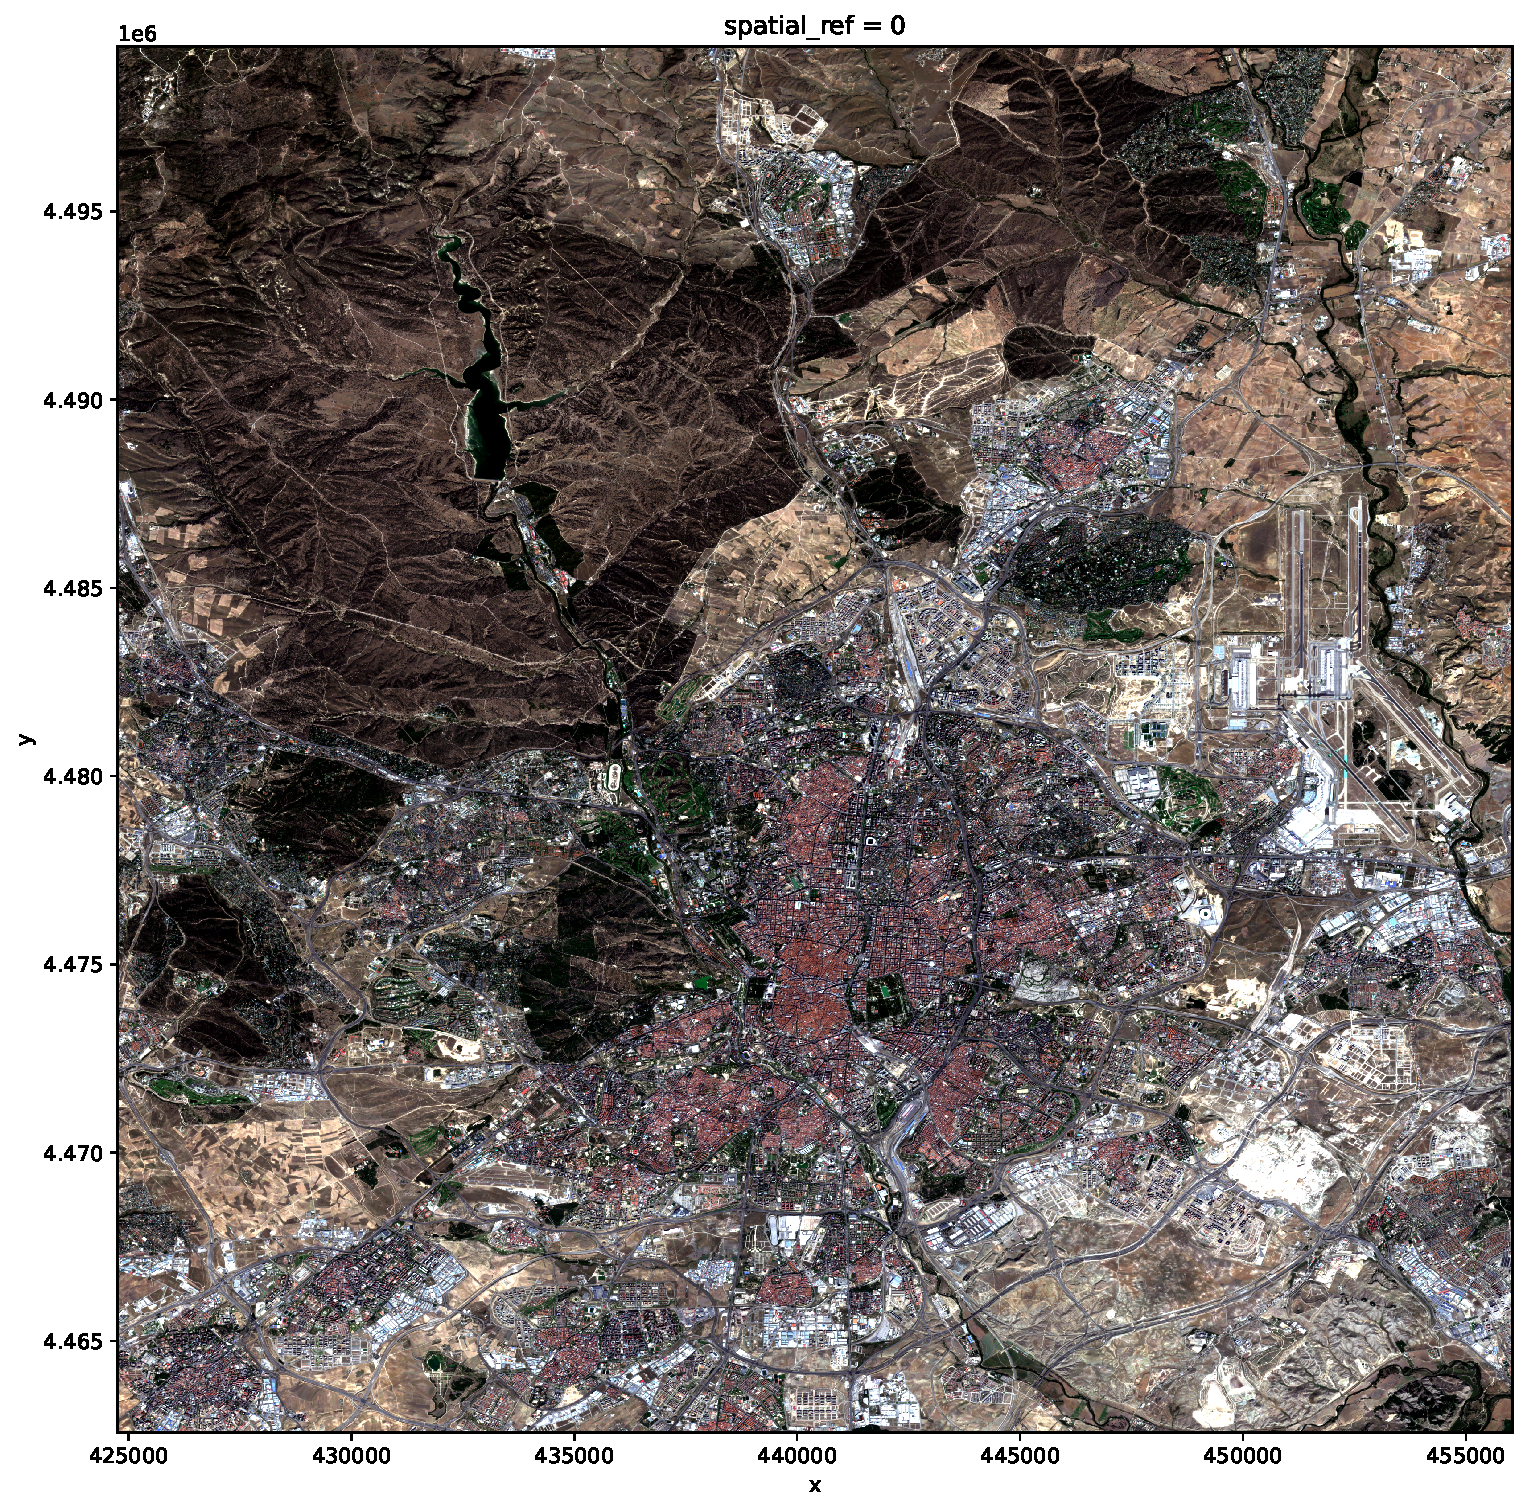
\includegraphics{mapvectorPy_files/figure-pdf/cell-21-output-1.pdf}

For example, the bin with highest values covers a much wider span that
the one with lowest, because there are fewer states in that value range.

You will notice a lot cooler difference once you play around with a
larger dataset.

\section*{Zooming into the map}\label{zooming-into-the-map}
\addcontentsline{toc}{section}{Zooming into the map}

\markright{Zooming into the map}

A general map of an entire region, or urban area, can sometimes obscure
local patterns because they happen at a much smaller scale that cannot
be perceived in the global view. One way to solve this is by providing a
focus of a smaller part of the map in a separate figure. Although there
are many ways to do this in \texttt{R}, the most straightforward one is
to define the bounding box.

As an example, let us consider the first \texttt{ggplot} map of this
Lab:

\subsection*{Zoom into full map}\label{zoom-into-full-map}
\addcontentsline{toc}{subsection}{Zoom into full map}

\begin{Shaded}
\begin{Highlighting}[]
\CommentTok{\# Setup the figure}
\NormalTok{f, ax }\OperatorTok{=}\NormalTok{ plt.subplots(}\DecValTok{1}\NormalTok{)}
\CommentTok{\# Draw the choropleth}
\NormalTok{world\_dev\_gdf.plot(}
\NormalTok{    column}\OperatorTok{=}\StringTok{"income\_group"}\NormalTok{, }
\NormalTok{    cmap}\OperatorTok{=}\StringTok{"YlGn"}\NormalTok{,}
\NormalTok{    legend}\OperatorTok{=}\VariableTok{True}\NormalTok{,}
\NormalTok{    ax}\OperatorTok{=}\NormalTok{ax}
\NormalTok{)}
\CommentTok{\# Redimensionate X and Y axes to desired bounds}
\NormalTok{ax.set\_ylim(}\FloatTok{30.520606}\NormalTok{, }\FloatTok{36.285000}\NormalTok{)}
\NormalTok{ax.set\_xlim(}\FloatTok{30.763478}\NormalTok{, }\FloatTok{40.332570}\NormalTok{)}

\CommentTok{\# Display image}
\NormalTok{plt.show()}
\end{Highlighting}
\end{Shaded}

\includegraphics{mapvectorPy_files/figure-pdf/cell-22-output-1.pdf}

\section*{Additional resources}\label{additional-resources-1}
\addcontentsline{toc}{section}{Additional resources}

\markright{Additional resources}

\begin{itemize}
\item
  On Drawing beautiful choropleths.html with \texttt{Python} and
  \texttt{ggplot} see
  \href{https://geopandas.org/en/stable/gallery/choropleths.html}{here}
\item
  If you want to have a look at \textbf{Choropleths in Python} have a
  look at the chapter on choropleth mapping by
  \href{https://geographicdata.science/book/notebooks/05_choropleth.html}{Rey,
  Arribas-Bel and Wolf}
\item
  Some more on mapping
  \href{https://geopandas.org/en/stable/docs/user_guide/mapping.html}{here}
\end{itemize}

\bookmarksetup{startatroot}

\chapter*{Data sets}\label{data-sets}
\addcontentsline{toc}{chapter}{Data sets}

\markboth{Data sets}{Data sets}

\bookmarksetup{startatroot}

\chapter*{References}\label{references}
\addcontentsline{toc}{chapter}{References}

\markboth{References}{References}

\phantomsection\label{refs}
\begin{CSLReferences}{0}{1}
\end{CSLReferences}




\end{document}
